
Trong chương này, tác giả trình bày tổng quan về hội chứng ngưng thở khi ngủ do
tắc nghẽn (OSA), phân tích ảnh hưởng của tư thế ngủ đối với mức độ nghiêm trọng
của OSA và dạng ngưng thở khi ngủ phụ thuộc tư thế (pOSA). Tiếp đó, chương tập
trung làm rõ cơ sở khoa học cho việc phát triển các thiết bị theo dõi giấc ngủ
và thiết bị HST (Home Sleep Test), nhận dạng tư thế ngủ tự động. Cuối cùng, tác
giả đưa ra xu hướng ứng dụng trí tuệ nhân tạo (AI) và điện toán biên (Edge
Computing) trong phân tích dữ liệu sinh lý và nhận dạng tư thế ngủ tự động, qua
đó đặt nền tảng cho các hướng nghiên cứu và triển khai kỹ thuật được trình bày
trong những chương tiếp theo.
\section{Hội chứng ngưng thở khi ngủ}

Trong lĩnh vực nghiên cứu các rối loạn hô hấp liên quan đến giấc ngủ, việc
chuẩn hóa và định nghĩa chính xác các kiểu sự kiện hô hấp giúp đảm bảo tính
nhất quán trong chẩn đoán, hỗ trợ phân tầng nguy cơ và lựa chọn phương pháp
điều trị phù hợp. Theo tiêu chuẩn chấm điểm của AASM \cite{berry2012scoring},
ba hiện tượng hô hấp chính cần được nhận diện bao gồm: ngưng thở (apnea), giảm
thở (hypopnea), và hiện tượng kích hoạt liên quan đến nỗ lực hô hấp
(Respiratory Effort–Related Arousal – RERA).

\subsection{Định nghĩa}

Ngưng thở (Apnea) được Hiệp hội Y học Giấc ngủ Hoa Kỳ (AASM) định nghĩa là sự
ngưng luồng khí hô hấp qua mũi và miệng trong thời gian tối thiểu 10 giây. Các
sự kiện ngưng thở có thể kéo dài đến 30 giây hoặc hơn trong những trường hợp
nặng. Có ba dạng chính của hội chứng ngưng thở khi ngủ \cite{ThaySYOSA}: ngưng
thở tắc nghẽn, ngưng thở trung ương, Ngưng thở hỗn hợp. Trong đó: 01)Ngưng thở
khi ngủ do tắc nghẽn (Obstructive Sleep Apnea – OSA) là dạng phổ biến nhất, xảy
ra khi các cơ vùng họng giãn ra và làm tắc đường thở, cản trở không khí đi vào
phổi \cite{osa_summary}; 02)Ngưng thở khi ngủ do trung ương (Central Sleep
Apnea – CSA) là tình trạng não không gửi tín hiệu đúng đến các cơ kiểm soát hô
hấp \cite{eckert2007csa}. 03)Ngưng thở hỗn hợp (Mixed Apnea) là sự kết hợp của
cả hai yếu tố: giai đoạn đầu của sự kiện không có nỗ lực hô hấp (giống CSA),
sau đó xuất hiện nỗ lực hô hấp (giống OSA). Dạng này thường xuất hiện ở những
bệnh nhân OSA nặng.

Giảm thở (Hypopnea) với hai mức tiêu chuẩn đánh giá: 01) Tiêu chuẩn khuyến
nghị: một sự kiện được xác định là hypopnea nếu thỏa mãn đồng thời ba điều
kiện: (i) biên độ tín hiệu luồng khí giảm $\geq 30$\% so với nền trước sự kiện,
đo bằng cảm biến áp lực mũi hoặc thiết bị CPAP; (ii) thời gian giảm tín hiệu
kéo dài $\geq 10$ giây; và (iii) kèm theo giảm độ bão hòa oxy $\geq 3$\%
và/hoặc gây kích hoạt điện não (arousal); 02) Tiêu chuẩn chấp nhận được
(Acceptable): tương tự như trên, tuy nhiên yêu cầu giảm độ bão hòa oxy phải đạt
từ 4\% trở lên.

RERA là sự kiện gia tăng nỗ lực hô hấp kéo dài $\geq 10$ giây, gây đánh thức
khỏi giấc ngủ nhưng không đủ tiêu chí của apnea hoặc hypopnea. 01) Phương pháp
tiêu chuẩn để đo là đo áp lực thực quản, tuy nhiên khó áp dụng do gây khó chịu
cho bệnh nhân. 02) Phương án thay thế đáng tin cậy là dùng ống thông mũi kết
hợp cảm biến áp lực, cho kết quả tương đương về mặt lâm sàng. 03) RERA được
tính vào chỉ số rối loạn hô hấp (Respiratory Disturbance Index - RDI); RDI >5
là bất thường, >15 là có ý nghĩa lâm sàng.

Trong số các rối loạn hô hấp liên quan đến giấc ngủ đã đề cập, hội chứng ngưng
thở khi ngủ do tắc nghẽn là dạng phổ biến nhất và có tác động sâu rộng đến sức
khỏe cộng đồng. Mức độ của OSA được đánh giá dựa trên chỉ số ngưng thở giảm thở
(Apnea–Hypopnea Index - AHI) bằng cách chia tổng số lần ngưng thở và giảm thở
cho tổng số giờ đã ngủ, với mỗi sự kiện phải kéo dài ít nhất 10 giây
Bảng~\ref{ahi} \cite{osa_summary}.
\begin{table}[h!]
  \caption{\texorpdfstring{Phân loại mức độ OSA dựa trên chỉ số AHI}{Phân loại OSA}}
  \label{ahi}
  \vspace{-3mm}
  \begin{center}
    \begin{tabular}{|c|c|}
      \hline
      AHI       & Cấp độ     \\
      \hline
      <5        & Không mắc  \\
      5 đến 10  & Nhẹ        \\
      15 đến 30 & Trung bình \\
      >30       & Nặng       \\
      \hline
    \end{tabular}
    \label{tab1}
  \end{center}
\end{table}

\subsection{Nguyên nhân}

Nguyên nhân chính của hội chứng OSA là do thu hẹp đường thở liên quan đến cấu
trúc hoặc phi cấu trúc, bao gồm cả yếu tố di truyền. Vì vậy, những người cao
tuổi, chỉ số khối cơ thể (Body mass Index - BMI) lớn, hoặc những người có tiển
sử bị các bệnh liên quan đến tim mạch, mỡ máu , tiểu đường sẽ có nguy cơ cao bị
mắc OSA \cite{wright1997health}. Tỷ lệ ngưng thở tắc nghẽn là từ 2\% đến 9\% ở
người lớn. Ngưng thở tắc nghẽn khi ngủ có thể tăng gấp 4 lần ở nam giới và gấp
7 lần hơn ở những người béo phì với BMI > 30. Ngoài ra, có thể đến từ thói quen
không lành mạnh của con người như là sử dụng các chất kích thích, hút thuốc,
ngáy khi ngủ \cite{reason_osa}\cite{reasonOsa}. Bên cạnh đó, các yếu tố không
giải phẫu như hoạt động kém của cơ giãn họng, ngưỡng thức giấc thấp và sự điều
hòa hô hấp không ổn định cũng góp phần quan trọng vào cơ chế bệnh sinh. Sự
tương tác giữa các yếu tố này tạo nên tính đa dạng trong biểu hiện và mức độ
nặng của OSA.

\subsection{Ảnh hướng của tư thế ngủ}

Đặc biệt, tư thế ngủ cũng là nguyên nhân có mối liên hệ chặt chẽ với mức độ nghiêm trọng của hội chứng OSA. Ở
tư thế nằm ngửa, tác động của trọng lực lên các cấu trúc mô mềm vùng hầu họng
làm tăng nguy cơ xẹp tắc đường thở trên, làm gia tăng tần suất các sự kiện
ngưng thở và giảm thở. Hội chứng ngưng thở khi ngủ tắc nghẽn tư thế (positional
Obstructive Sleep Apnea – pOSA) là một thể đặc biệt của OSA, trong đó mức độ
nghiêm trọng của rối loạn hô hấp phụ thuộc đáng kể vào tư thế ngủ của bệnh
nhân. Về mặt chẩn đoán, pOSA được xác định khi chỉ số ngưng thở – giảm thở
(Apnea–Hypopnea Index, AHI) trong tư thế nằm ngửa cao hơn rõ rệt so với các tư
thế khác, thường gặp ở bệnh nhân OSA mức độ nhẹ đến trung bình
\cite{heinzer2018,aloweidat2023positional}.

Các nhà nghiên cứu đã đề xuất nhiều tiêu chí khác nhau nhằm chẩn đoán pOSA, từ
đơn giản đến phức tạp. Định nghĩa cổ điển nhất được giới thiệu bởi Cartwright,
theo đó bệnh nhân được coi là pOSA nếu AHI ở tư thế nằm ngửa lớn hơn ít nhất
hai lần so với AHI ở tư thế không nằm ngửa \cite{cartwright1984position}. Mador
sau đó kế thừa định nghĩa này và bổ sung tiêu chí rằng AHI ở tư thế không nằm
ngửa phải nhỏ hơn 5 lần/giờ, nhằm tăng tính đặc hiệu trong chẩn đoán
\cite{mador2005prevalence}. Song song đó, Levendowski đề xuất một cách tiếp cận
theo tỷ lệ, trong đó pOSA được xác định khi AHI toàn bộ lớn hơn hoặc bằng 1.5
lần AHI ở tư thế không nằm ngửa \cite{levendowski2015neck}. Một phương pháp
phân loại với các bệnh nhân có chỉ số AHI cao là Amsterdam Positional
Obstructive Sleep Apnea Classification (APOC) \cite{frank2014positional}. Tiêu
chí APOC xác định pOSA khi bệnh nhân có AHI toàn bộ lớn hơn 5 lần/giờ, đồng
thời tổng thời gian ngủ (Total Sleep Time – TST) ở tư thế tốt nhất (Best
Sleeping Position – BSP) và tư thế gây ra chỉ số AHI cao nhất (Worst Sleeping
Position – WSP) đều chiếm tối thiểu 10\% TST. Qua đó, chia làm ba nhóm nhóm
APOC-I bao gồm bệnh nhân có thể khỏi hoàn toàn nhờ thay đổi tư thế; nhóm
APOC-II là không phụ thuộc vào tư thế và APOC-III có phụ thuộc một phần.

\subsection{Ảnh hưởng của OSA}
Ngưng thở khi ngủ có thể gây ra những hậu quả đáng kể về thần kinh, tim mạch và
chuyển hóa. OSA là nguyên nhân y khoa hàng đầu gây ra tình trạng buồn ngủ quá
mức vào ban ngày. Tình trạng buồn ngủ quá mức làm tăng nguy cơ bị tai nạn ô tô,
khó khăn trong công việc và rối loạn chức năng tình dục
\cite{flemons1997quality}. Tình trạng hạ oxy trong máu về đêm lặp đi lặp lại và
gián đoạn giấc ngủ có làm tăng nguy cơ mắc các bệnh lý, bao gồm suy tim, bệnh
động mạch vành, và các loạn nhịp khác, bệnh gan nhiễm mỡ liên quan đến rối loạn
chuyển hóa và đột quỵ \cite{ wright1997health,Zinchuk2018,
  young1997population}.
\subsection{Chẩn đoán OSA}
Phần lớn bệnh nhân mắc hội chứng ngưng thở khi ngủ tắc nghẽn (\gls{OSA}) không
tự nhận thức được các rối loạn hô hấp xảy ra trong lúc ngủ. Điều này đặc biệt
đúng với những người sống hoặc ngủ một mình, do thiếu sự quan sát từ bên ngoài.
Đáng lưu ý, hơn 80\% các trường hợp OSA được phát hiện ở những bệnh nhân mắc
các bệnh lý liên quan đến béo phì như tiểu đường, bệnh thận, rối loạn lipid
máu.

Trong điều kiện hiện tại, đa số bệnh nhân nghi ngờ mắc hội chứng ngưng thở tắc
nghẽn khi ngủ được khám bới bs chuyên khoa Tai Mũi Họng và bác sĩ chuyên gia về
ngủ ngáy. Khám tổng quát kết hợp khai thác bệnh sử liên quan, sử dụng các thang
điểm đánh giá buồn ngủ và nguy cơ ngưng thở khi ngủ, như Epworth Sleepiness
Scale, STOP-BANG được chấp thuận tại Việt Nam như một phương án sáng lọc bệnh
nhân OSA hoặc có thể khám nội soi Tai Mũi Họng để tìm nguyên nhân. Vì đa số các
trường hợp ngáy, ngưng thở khi ngủ nguyên nhân từ mũi, họng, amidan, và những
bất thường về hàm mặt khác. Việc đánh giá ngưng thở khi ngủ bắt đầu thường bắt
đầu bằng một khảo sát giấc ngủ toàn diện, bao gồm khai thác bệnh sử liên quan
đến các triệu chứng lâm sàng đặc trưng, sau đó tiến hành đánh giá khách quan
thông qua đa ký giấc ngủ (Polysomnography - PSG)
\cite{diagnosis_osa}\cite{medical2006polysomnography}.

Phương pháp do dùng đa ký giấc ngủ với sự giám sát của các bác sĩ chuyên môn
được coi là tiêu chuẩn vàng trong chẩn đoán chứng ngưng thở khi ngủ. PSG là một
phương pháp ghi đa kênh liên tục trong suốt một đêm, bao gồm nhiều thông số
sinh lý nhằm đánh giá toàn diện hoạt động hô hấp và thần kinh khi ngủ. Các
thành phần chính trong một đánh giá polysomnography bao gồm: điện não đồ (EEG)
để ghi lại hoạt động điện của não; điện cơ ký (EMG) nhằm đo trương lực cơ, đặc
biệt là ở cằm và chân; điện động mắt (EOG) để theo dõi chuyển động của nhãn
cầu, giúp xác định các giai đoạn của giấc ngủ; và điện tâm đồ (ECG) để theo dõi
hoạt động điện của tim. Bên cạnh đó, quá trình đo cũng bao gồm theo dõi độ bão
hòa oxy trong máu (SpO$_2$), đo lưu lượng khí thở qua mũi và miệng, đánh giá nỗ
lực hô hấp thông qua chuyển động của ngực và bụng, đo áp lực khí thở qua mũi,
và ghi nhận cường độ tiếng ngáy. Tư thế ngủ là một tín hiệu quan trọng trong
polysomnography (PSG), đặc biệt có giá trị trong chẩn đoán và phân loại hội
chứng ngưng thở khi ngủ tắc nghẽn phụ thuộc tư thế (positional OSA – pOSA).
Trong quá trình ghi đa ký giấc ngủ, việc theo dõi liên tục tư thế cơ thể giúp
xác định mối liên hệ giữa tư thế nằm với tần suất và mức độ nghiêm trọng của
các rối loạn hô hấp. Tập hợp các thông số này sẽ được lưu trữ, cho phép bác sĩ
chẩn đoán chính xác hội chứng ngưng thở khi ngủ tắc nghẽn (OSA).

Một trong những hạn chế của phương pháp đánh giá sử dụng (\gls{PSG}) là sự bất
tiện, chi phí cao, thời gian chờ, nhất là đối với phần lớn người bệnh có thu
nhập thấp. Việc yêu cầu bệnh nhân phải lưu trú qua đêm tại cơ sở y tế, cùng với
việc gắn nhiều thiết bị theo dõi sinh lý lên cơ thể có thể một phần nào làm sai
lệnh so với hàng ngày. Theo khảo sát của chính tác giả, rất nhiều ca thu thập
bị ngắt quãng tín hiệu, hoặc thiếu hẳn một số tín hiệu. Tuy nhiên, thực tế với
kinh nghiệm của mình các bác sĩ có những phương pháp để nhận dạng bất thường từ
đặc trưng tín hiệu - đây chính là ý tưởng để triển khai các bài toán học máy.
Chính những bất cập này đã thúc đẩy sự phát triển của các thiết bị theo dõi
giấc ngủ ngoài trung tâm (Out-of-Center devices) hay còn gọi là thiết bị kiểm
tra giấc ngủ tại nhà (Home Sleep Test – HST). Những thiết bị này thường được
thiết kế với số lượng cảm biến tối giản hơn so với PSG truyền thống, đồng thời
tích hợp các thuật toán phân tích tự động – được xử lý trực tiếp trên thiết bị
hoặc thông qua phần mềm chuyên dụng – nhằm hỗ trợ chẩn đoán OSA một cách thuận
tiện và tiết kiệm hơn. Nhưng thông số SCOPERA được coi là cơ sở để xây dựng
thiết bị HST trong đó giấc ngủ (Sleep - S), tim mạch (Cardiovascular - C), oxi
trong máu (Oximetry - O), cố gắng thở (Effort - E), luồng không khí lưu thông
(Respiratory - R), âm thở (Audio - A).

\section{Công nghệ trong đánh giá OSA và phân loại tư thế ngủ}

Như đã trình bày ở phần trước, xu hướng sử dụng các thiết bị HST trước khi đánh
giá chính xác bằng PSG đang gia tăng đáng kể bởi sử tiện dụng, chi phí thấp. Về
mặt kỹ thuật, các thiết bị hiện đại thường dựa trên việc thu thập và phân tích
các tín hiệu sinh lý như hô hấp, nhịp tim, độ bão hòa oxy máu và gia tốc ba
trục . Dữ liệu thu được được xử lý thông qua các mô hình toán học hoặc thuật
toán học máy, cho phép đánh giá mức độ OSA cũng như phân loại tư thế ngủ với độ
chính xác cao. Cách tiếp cận này là nền tảng cho xu hướng phát triển các hệ
thống đánh giá OSA thông minh, có khả năng hoạt động theo thời gian thực và
không phụ thuộc vào kết nối internet.

\subsection{Công nghệ trong đánh giá OSA}

Thiết bị đeo hỗ trợ theo dõi giấc ngủ đang trở thành một xu hướng chủ đạo trong
nghiên cứu và ứng dụng lâm sàng nhờ khả năng thu thập liên tục dữ liệu sinh lý
một cách không xâm lấn, thuận tiện và có thể triển khai tại nhà. Dựa trên đặc
điểm hình thái và vị trí gắn trên cơ thể, các thiết bị này có thể được phân
thành các nhóm: vòng tay, đai ngực, miếng dán, tai nghe, nhẫn thông minh Bảng
\ref{tab:wearable_types}.

Jeon và cộng sự \cite{jeon2020realtime} Nghiên cứu sử dụng thiết bị đeo Sleep
Care Kit gắn ở ngực để thu thập các tín hiệu nhịp tim, gia tốc ba trục, hô hấp
và nồng độ oxy trong máu. Các mô hình Gaussian Naive Bayes, Artificial Neural
Network và k-Nearest Neighbor được huấn luyện nhằm phân loại trạng thái hô hấp
– ngưng thở. Kết quả cho thấy mô hình KNN đạt độ chính xác 95\% và thời gian xử
lý 640~$\mu$s, đáp ứng yêu cầu chẩn đoán OSA theo thời gian thực. Trong nghiên
cứu \cite{chen2024hdc}, Chen và cộng sự sử dụng thiết bị đeo dạng vòng tay thu
tín hiệu PPG để phát hiện ngưng thở khi ngủ ở 100 tình nguyện viên. Thiết bị
được thiết kế tối ưu về bộ nhớ, độ trễ và năng lượng, phù hợp triển khai trên
các hệ thống tính toán giới hạn. Dữ liệu thu được được đồng bộ với PSG nhằm đảm
bảo độ chính xác, đồng thời hướng tới ứng dụng giám sát dài hạn tại nhà. Trong
các nghiên cứu \cite{yeo2022resnet, yeo2022respiratory}, Yeo và cộng sự sử dụng
thiết bị dán T-REX TR100A để ghi điện tâm đồ (ECG) một kênh từ vùng bụng trên.
Thiết bị được dán trực tiếp lên da, đảm bảo tiếp xúc ổn định và tín hiệu thu
nhận chính xác, giúp theo dõi liên tục và hạn chế nguy cơ bị bong tróc trong
quá trình sử dụng. Một thiết bị HST dạng miếng dán cổ đã được phát triển, tích
hợp cảm biến gia tốc ba trục LIS2DH12 và vi điều khiển nRF5232, cho phép truyền
dữ liệu không dây qua Bluetooth Low Energy (BLE) với tần số lấy mẫu 100~Hz
\cite{Sleep_Posture_Detection}. Thiết bị có kích thước nhỏ gọn
(\textasciitilde3207~mm\textsuperscript{3}), được dán trực tiếp lên vùng cổ
bằng băng dính hai mặt, giúp đảm bảo tiếp xúc ổn định với da. Thiết kế này cho
phép ghi nhận chính xác các tư thế ngủ phổ biến như nằm ngửa, nằm nghiêng và
nằm sấp, phù hợp với mục tiêu theo dõi tại nhà và hỗ trợ đánh giá nguy cơ mắc
pOSA. Nghiên cứu\cite{svmHSt2017} chứng minh rằng tín hiệu chuyển động ngực
(Thoracic movement signal - THO) và bụng (Abdominal movement signal - ABD), thu
từ các dải piezoelectric đeo được, có thể được sử dụng hiệu quả để phân loại
các dạng rối loạn thở khi ngủ thông qua mô hình thuật toán SVM. Kết quả cho
thấy khi kết hợp cả hai tín hiệu, độ chính xác phân loại đạt trung bình 81.8\%,
khẳng định tiềm năng ứng dụng của phương pháp này trong sàng lọc và theo dõi
OSA tại nhà hoặc trong lâm sàng. Gần đây, Domingues và cộng sự (2024) xây dựng
một mô hình mạng nơ-ron nhân tạo dựa trên dữ liệu từ máy đo (SpO$_2$), cấm biến
gia tốc và ghi âm tiếng ngáy của hệ thống Biologix, nhằm dự đoán chính xác
trạng thái ngủ. Kết quả cho thấy mô hình này có khả nâng cao độ chính xác trong
chẩn đoán ngưng thở khi ngủ tại nhà, tiệm cận với tiêu chuẩn của đa ký giấc ngủ
truyền thống \cite{domingues2024sleep}. Một hướng nghiên cứu khác là cảm biến
đặt dưới nệm giường. Tác giả Andrei Boiko và cộng sự đánh giá hệ thống phát sử
dụng cảm biến gia tốc đặt dưới đệm giường để ghi dao động do cử động ngực khi
thở. Kết quả cho thấy thuật toán phát hiện ngưng thở đạt độ chính xác, độ đặc
hiệu và độ nhạy lần lượt là 94.6\%, 95.3\% và 93.7\% \cite{Boiko2023}.

\begin{table}[htbp]
  \centering
  \caption{Phân loại thiết bị đeo trong phát hiện OSA. tư thế ngủ}
  \label{tab:wearable_types}
  \begin{tabular}{|p{5.5cm}|p{7.5cm}|}
    \hline
    \textbf{Loại thiết bị đeo} & \textbf{Tài liệu tham khảo}                                                                                                          \\
    \hline
    Vòng tay                   & \cite{jeon2020realtime}, \cite{shen2022mtcnn} \cite{e3hst} \cite{osa_sanchez2025}                                                    \\
    \hline
    Đai ngực                   & \cite{svmHSt2017}, \cite{chen2024hdc} \cite{e3hst} \cite{osa_sanchez2025}                                                            \\
    \hline
    Miếng dán                  & \cite{Vu2025SleepPosition}, \cite{yeo2022resnet}, \cite{yeo2022respiratory}, \cite{p_3} \cite{osa_sanchez2025}                       \\
    \hline
    Dạng khác                  & \cite{Sleep_Posture_Detection}, \cite{hst_wear_paper} \cite{osa_sanchez2025} \cite{hstSurvey} \cite{hst_paper} \cite{hst_wear_paper} \\
    \hline
  \end{tabular}
\end{table}

Tuy nhiên, một rào cản lớn cho việc triển khai HST trên diện rộng vẫn nằm ở chi
phí. Theo báo cáo tổng quan \cite{hst_review}, giá trung bình của một thiết bị
HST khoảng 2300 USD – vượt quá khả năng chi trả của đại đa số bệnh nhân, đặc
biệt ở các nước có thu nhập trung bình – thấp. Do đó, việc tối ưu hóa chi phí,
giảm số lượng cảm biến và đơn giản hóa quy trình sử dụng vẫn là các mục tiêu
cấp thiết.

Hiện nay, đã có nhiều nghiên cứu và sản phẩm thương mại được phát triển nhằm
mục đích theo dõi tư thế ngủ. Trong đó, iSleePost là một hệ thống thiết bị đeo
được phát triển bởi Po-Yuan Jeng và cộng sự \cite{Jeng}, gồm hai thiết bị đeo
độc lập sử dụng cảm biến gia tốc để theo dõi và phân loại tư thế ngủ. Trong đó,
một thiết bị được đeo ở cổ tay nhằm ghi nhận chuyển động, còn thiết bị thứ hai
được gắn ở ngực để thu thập nhãn tư thế một cách tự động phục vụ huấn luyện mô
hình. Dữ liệu từ cổ tay được xử lý bằng kỹ thuật cửa sổ trượt để trích xuất đặc
trưng, sau đó ánh xạ với tư thế cơ thể dựa trên dữ liệu từ thiết bị ngực. Một
hướng tiếp cận khác, Zhang và cộng sự sử dụng duy nhất một thiết bị đeo gắn ở
ngực, có tích hợp cảm biến gia tốc ba trục, để theo dõi cả tư thế ngủ và các
chỉ số sinh lý như nhịp tim và nhịp thở \cite{Zhang_osa}. Trong nghiên cứu được
thực hiện trên 7 tình nguyện viên khỏe mạnh trong điều kiện phòng lab, hệ thống
sử dụng bộ phân loại tuyến tính (LDA) để nhận diện bốn tư thế ngủ phổ biến
trong trạng thái tĩnh, kết hợp với thuật toán phát hiện chuyển động hiệu quả
nhằm phân biệt giữa tư thế tĩnh và vận động. Một hệ thống thiết bị đeo theo dõi
tư thế ngủ (Wearable Sleep System – WSS), được Kwasnicki và cộng sự phát triển
với thiết kế riêng biệt, gồm các cảm biến đeo trên mỗi cánh tay và vùng ngực,
kết nối không dây với bộ xử lý trung tâm (trong nghiên cứu là máy tính xách
tay) thông qua bộ thu phát sóng vô tuyến \cite{kwasnicki2018}. Nền tảng phần
cứng của hệ thống sử dụng bộ vi xử lý tiêu thụ điện năng cực thấp TI MSP430,
kết hợp với mô-đun truyền thông không dây Chipcon CC2420, cùng pin Li-ion
polymer nhẹ. Mỗi nút cảm biến được tích hợp cảm biến gia tốc ba trục ADXL330,
con quay hồi chuyển số ITG-3200, và cảm biến từ trường ba trục HMC5843. Toàn bộ
mô-đun có kích thước 20×30×17 mm, trọng lượng 10 g. Trong nghiên cứu của Asma
Channa và cộng sự \cite{Channa_osa}, một hệ thống theo dõi tư thế ngủ dựa trên
công nghệ Internet vạn vật (IoT) đã được đề xuất, sử dụng hai thảm cảm biến áp
lực thương mại để thu thập dữ liệu từ 13 người tham gia ở các tư thế ngủ khác
nhau. Dữ liệu được xử lý bằng nhiều thuật toán học máy giám sát, trong đó các
mô hình như Weighted KNN và Linear SVM đạt độ chính xác nhận dạng tư thế lên
tới 98,7\%.

Các nghiên cứu hiện nay đã phát triển nhiều hệ thống theo dõi tư thế ngủ với độ
chính xác cao, sử dụng đa dạng nền tảng như thiết bị đeo tích hợp cảm biến gia
tốc, PPG, ECG hoặc thảm cảm biến áp lực. Nhiều hệ thống đã chứng minh hiệu quả
trong việc phân loại tư thế ngủ và ghi nhận các chỉ số sinh lý liên quan đến
hội chứng ngưng thở khi ngủ tắc nghẽn (OSA).

Tuy nhiên, để đáp ứng yêu cầu triển khai thực tế tại nhà, các giải pháp cần
được tiếp tục hoàn thiện theo hướng tối giản phần cứng, giảm số lượng cảm biến,
đồng thời tối ưu mô hình học máy cho nền tảng tính toán giới hạn (TinyML). Việc
xây dựng một quy trình thu thập và xử lý dữ liệu rõ ràng, có thể lặp lại, cũng
đóng vai trò quan trọng trong việc đảm bảo tính ổn định và khả năng áp dụng
rộng rãi.

Bám sát định hướng này, luận văn đề xuất một hệ thống sử dụng duy nhất một cảm
biến gia tốc dán dưới hõm ức để phát hiện các tư thế ngủ liên quan đến OSA.
Trên cơ sở dữ liệu thu được, mô hình học máy nhẹ sẽ được xây dựng và tối ưu,
hướng tới việc phát triển thiết bị IoT nhỏ gọn, chi phí thấp, có khả năng ước
lượng chỉ số AHI – phục vụ cho sàng lọc và theo dõi OSA tại nhà một cách hiệu
quả.

\section{Ứng dụng cảm biến gia tốc trong đánh giá tư thế ngủ của người mắc OSA tại nhà}

Tư thế ngủ của con người thường được phân loại thành bốn nhóm chính: nằm ngửa,
nghiêng trái, nghiêng phải và nằm sấp (Hình~\ref{4_tuthe}) \cite{4_ngu}. Việc
phân biệt rõ ràng các tư thế này giúp nâng cao độ chính xác trong việc phân
tích ảnh hưởng của tư thế đến các chỉ số sinh lý trong giấc ngủ.

\begin{figure}
  \centering
  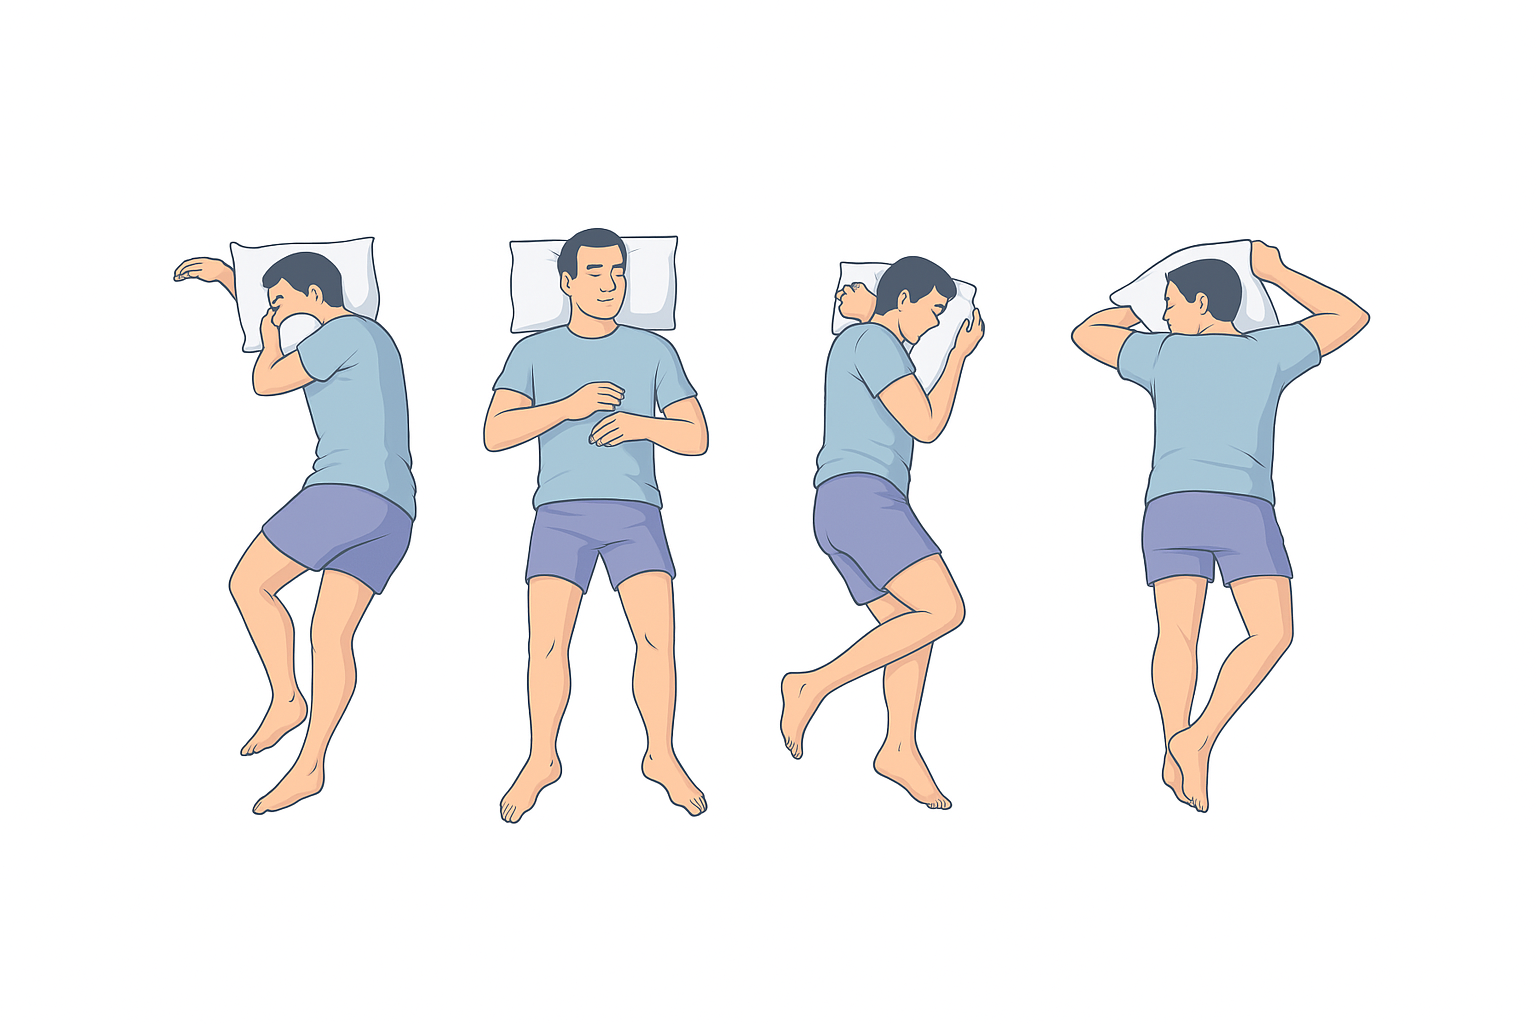
\includegraphics[width=\textwidth]{images/4ngu.png}
  \vspace*{-7mm}
  \caption{Các tư thế ngủ cơ bản của con người}
  \label{4_tuthe}
\end{figure}

Việc theo dõi tư thế cơ thể đặc biệt hữu ích trong phát hiện và điều trị hội
chứng ngưng thở khi ngủ phụ thuộc tư thế (positional OSA). Hiểu được mối quan
hệ giữa tư thế ngủ và rối loạn hô hấp sẽ mở ra hướng điều trị cá thể hóa, chẳng
hạn như liệu pháp định hướng tư thế.

Trong bối cảnh đó, cảm biến gia tốc ba trục (triaxial accelerometers) nổi lên
như một công cụ đầy hứa hẹn nhờ vào đặc tính đo lường trực tiếp chuyển động và
hướng trọng lực của cơ thể. So với các phương pháp truyền thống như ghi hình
hồng ngoại, cảm biến áp suất hay hệ thống camera đa góc, gia tốc kế mang lại ưu
thế về kích thước, mức độ xâm nhập, khả năng tiêu thụ năng lượng thấp và đặc
biệt là chi phí triển khai hợp lý – các yếu tố quyết định khi xét đến ứng dụng
tại nhà trên quy mô lớn.

Các hệ thống ghi hình sử dụng camera hồng ngoại có khả năng ghi nhận toàn bộ
hoạt động của cơ thể trong điều kiện ánh sáng yếu, và có thể kết hợp với học
sâu để phân loại tư thế ngủ một cách chính xác. Tuy nhiên, phương pháp này đòi
hỏi không gian phòng ngủ cố định, điều kiện lắp đặt tối ưu, và đặt ra các thách
thức về quyền riêng tư \cite{Akbarian_osa}. Việc tái tạo các góc khuôn mặt hoặc
cơ thể khi bị chăn/mền che khuất cũng làm giảm hiệu quả hệ thống. Trong khi đó,
cảm biến áp suất bố trí dưới đệm có thể ghi nhận phân bố trọng lực và áp lực
tiếp xúc, từ đó gián tiếp suy đoán tư thế. Channa và cộng sự \cite{Channa_osa}
sử dụng tới 2048 điểm cảm biến để tăng cường độ phân giải, cho phép phân biệt
chính xác các tư thế cơ bản. Tuy nhiên, nhược điểm của phương pháp này nằm ở
tính cố định (không đeo được), chi phí lắp đặt cao và không phù hợp cho người
hay di chuyển nơi ngủ hoặc sinh sống trong điều kiện không gian hạn chế.

Trái lại, cảm biến gia tốc mang tính linh hoạt cao. Thiết bị có thể đeo trực
tiếp lên cơ thể (dạng vòng tay, miếng dán, đai ngực) hoặc tích hợp vào các vật
dụng quen thuộc như điện thoại di động \cite{sun2017sleepmonitor, Natale_osa}.
Thiết kế này vừa đảm bảo tính di động, vừa cho phép giám sát liên tục với mức
độ can thiệp tối thiểu.

Từ góc độ học thuật, các nghiên cứu gần đây đã xác nhận hiệu quả của cảm biến
gia tốc trong phân loại tư thế ngủ. Jeng và công sự \cite{Jeng} sử dụng thiết
bị đeo tay kết hợp cảm biến ngực để huấn luyện mô hình học máy đạt độ chính xác
trên 85\%. Zhang và cộng sự \cite{Zhang_osa} chỉ sử dụng một cảm biến tại vị
trí xương ức đã có thể phân biệt chính xác các tư thế phổ biến. Đặc biệt, việc
chọn vị trí gắn cảm biến là yếu tố then chốt. Các vị trí như cổ tay hay trán
thường chịu nhiều chuyển động ngoại ý và lệch trục so với thân người, làm giảm
tính đại diện của tín hiệu. Vùng xương ức, cụ thể là ngay dưới hõm cổ
(suprasternal notch), được xem là vị trí lý tưởng do sự ổn định hình học và gần
đường trung trục cơ thể, từ đó phản ánh đúng hướng trọng lực – nền tảng để suy
luận tư thế một cách chính xác.

Ngoài ra, hiện nay với sự phát triển vượt bậc của điện thoại di động, việc tận
dụng cảm biến gia tốc ở ngay trên chính chiếc điện thoại cũng là giải pháp hữu
hiệu \cite{sun2017sleepmonitor}. Nhóm tác giả trong \cite{Ferrer_osa} đã báo
cáo nghiên cứu đánh giá tư thế ngủ của bệnh nhân sử dụng thiết bị di động đeo ở
xương ức kết hợp với phần mềm trên nền tảng Android để thu thập lại dữ liệu kể
cả khi tắt màn hình. Trong một nghiên cứu tiêu biểu, Natale và cộng sự đã khai
thác các cảm biến tích hợp sẵn trên điện thoại iPhone để ước lượng các thông số
liên quan đến chất lượng giấc ngủ, bao gồm tổng thời gian ngủ (Total Sleep Time
– TST), độ trễ vào giấc (Sleep Onset Latency – SOL) và hiệu quả giấc ngủ (Sleep
Efficiency – SE). Phương pháp tiếp cận này cho thấy tiềm năng trong việc sử
dụng thiết bị di động như một công cụ theo dõi giấc ngủ tiện lợi và dễ tiếp
cận, đặc biệt trong các nghiên cứu cộng đồng và ứng dụng tại
nhà\cite{Natale_osa}. Đặc điểm của sử dụng tích hợp cảm biến gia tốc trên điện
thoại là rất tiện lợi, sử dụng trực tiếp mà không cần phát triển phần cứng. Tuy
nhiên, việc tiếp xúc điện thoại trực tiếp với cơ thể trực tiếp trong thời gian
lâu cũng có gây những ảnh hưởng nhất định đến người dùng.

\begin{figure}[!ht]
  \centering
  % 		\setlength{\abovecaptionskip}{1pt plus 3pt minus 2pt}
  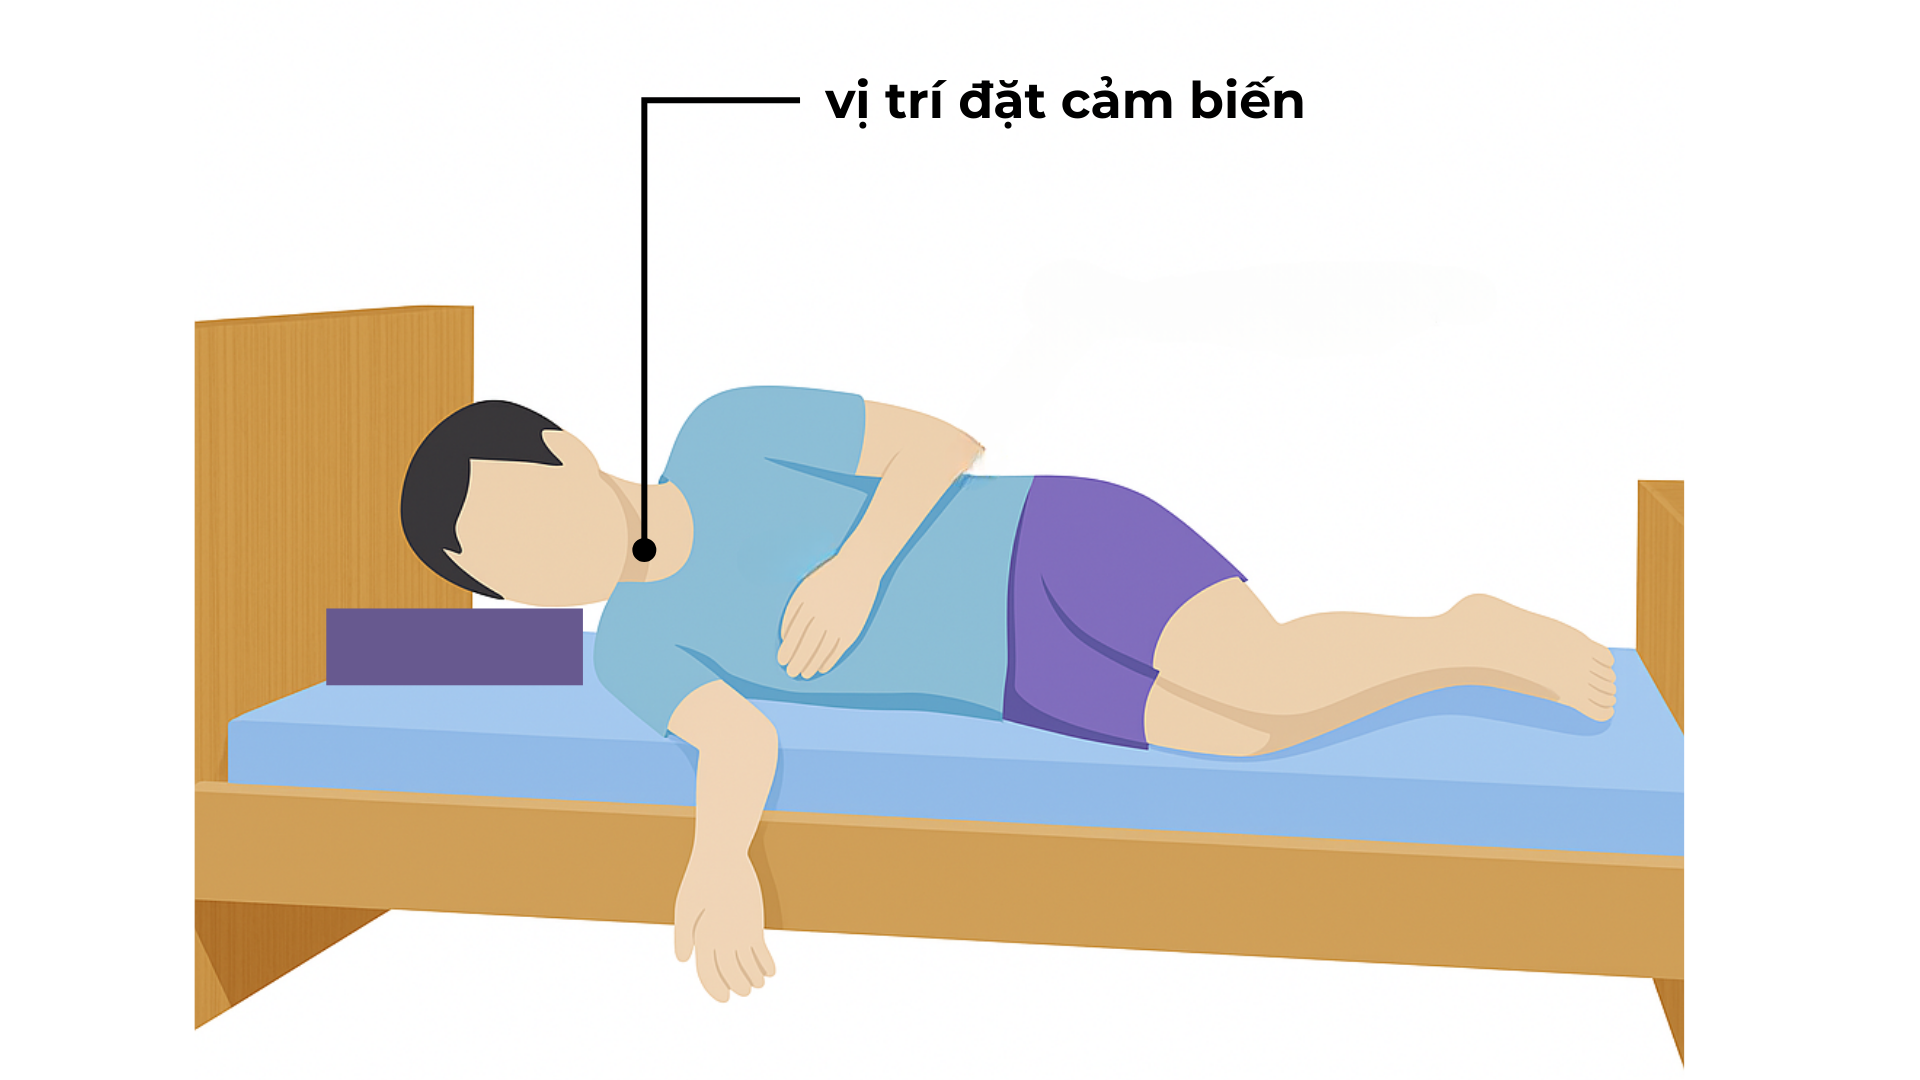
\includegraphics[width=\textwidth]{images/vị trí đặt cảm biến.png}
  \vspace*{-7mm}
  \caption{Vị trí tối ưu để đặt cảm biến gia tốc}
  \label{position_sensor}
\end{figure}

Ưu điểm nổi bật nhất của cảm biến gia tốc là khả năng hoạt động độc lập
với mức tiêu thụ điện năng thấp, dễ dàng tích hợp vào hệ thống vi điều
khiển nhúng như nRF52, ESP32, hoặc STM32 để xây dựng thiết bị đeo có khả
năng xử lý cục bộ (on-device) – phù hợp với định hướng TinyML.
Ngoài ra, cảm biến gia tốc không yêu cầu điều kiện môi trường đặc
biệt như ánh sáng hay bề mặt phẳng, đồng thời không ảnh hưởng đến
quyền riêng tư như hệ thống camera.

Tuy nhiên, giới hạn của cảm biến gia tốc là việc nhận diện tư thế phụ thuộc
mạnh vào vị trí gắn cảm biến. Một cảm biến đặt sai vị trí hoặc xoay lệch trục
có thể làm sai lệch hoàn toàn kết quả phân loại. Hơn nữa, gia tốc kế không cung
cấp thông tin về các chỉ số sinh lý như $\mathrm{SpO_2}$, nhịp thở hay nhịp
tim, vì vậy để chẩn đoán toàn diện OSA, cần tích hợp thêm các cảm biến khác
hoặc kết hợp với các mô hình suy luận (inference models) để bù đắp cho thiếu
sót này.
\begin{table}[htbp]
  \centering
  \caption{So sánh ưu và nhược điểm của các vị trí gắn cảm biến gia tốc trong theo dõi tư thế ngủ}
  \label{tab:sensor_position}
  \small
  \renewcommand{\arraystretch}{1.3}
  \begin{tabular}{|p{3cm}|p{5.2cm}|p{6.2cm}|}
    \hline
    \textbf{Vị trí}                                                      & \textbf{Ưu điểm} & \textbf{Nhược điểm} \\
    \hline
    \textbf{Cổ tay}                                                      &
    - Dễ đeo, quen thuộc (giống đồng hồ, vòng tay).
    - Thuận tiện cho người dùng tự gắn.                                  &
    - Chịu nhiều chuyển động ngoài ý muốn của tay.
    - Tín hiệu kém đại diện cho tư thế toàn thân.                                                                 \\
    \hline
    \textbf{Trán}                                                        &
    - Có thể cố định bằng băng quấn đầu.
    - Ít bị ảnh hưởng bởi quần áo hay chăn phủ.                          &
    - Không phản ánh chính xác trục cơ thể.
    - Gây khó chịu, ảnh hưởng thẩm mỹ và giấc ngủ.                                                                \\
    \hline
    \textbf{Ngực (lateral)}                                              &
    - Gần trung tâm thân người, phản ánh tương đối hướng trọng lực.
    - Thuận lợi để kết hợp với dây đeo ngực (chest strap).               &
    - Có nguy cơ xô lệch khi nằm nghiêng.
    - Có thể gây khó chịu khi nằm sấp.                                                                            \\
    \hline
    \textbf{Xương ức (suprasternal notch)}                               &
    - Ổn định hình học, gần trục trung tâm cơ thể.
    - Phản ánh chính xác hướng trọng lực và tư thế toàn thân.
    - Ít chịu ảnh hưởng từ chuyển động tay/chân.
    - Thuận lợi để tích hợp thêm cảm biến (âm thanh, nhiệt độ, SpO$_2$). &
    - Yêu cầu thiết kế miếng dán/thiết bị đeo chuyên dụng để cố định đúng vị trí.                                 \\
    \hline
  \end{tabular}
\end{table}

Xuất phát từ các phân tích nêu trên, nghiên cứu này lựa chọn thiết kế một thiết
bị đeo tiếp xúc sử dụng cảm biến gia tốc ba trục, được gắn tại vùng xương ức
(suprasternal notch). Việc lựa chọn vị trí và cấu trúc thiết bị được cân nhắc
dựa trên các yếu tố sau (Hình~\ref{position_sensor}).
Bảng~\ref{tab:sensor_position} dưới đây so sánh ưu và nhược điểm của các vị trí
gắn cảm biến gia tốc thường gặp, qua đó cho thấy vùng xương ức (suprasternal
notch) là lựa chọn hợp lý nhất:

\begin{enumerate}
  \item Vị trí xương ức có độ ổn định cao trong suốt quá trình ngủ, hạn chế dịch chuyển
        ngoài ý muốn, từ đó đảm bảo tính nhất quán của dữ liệu thu nhận.
  \item Vị trí này phản ánh chính xác hướng trọng lực của cơ thể, giúp tăng độ chính
        xác trong phân loại tư thế ngủ dựa trên gia tốc ba trục (x, y, z).
  \item Cấu trúc gắn tại xương ức thuận lợi cho việc tích hợp thêm các cảm biến khác
        như cảm biến âm thanh (microphone) hoặc cảm biến nhiệt độ, phục vụ cho các mục
        tiêu mở rộng trong các nghiên cứu tiếp theo.
\end{enumerate}

Sau khi xác định được vị trí gắn tối ưu, bước tiếp theo là làm rõ cơ sở nguyên
lý đo lường của cảm biến, nhằm lý giải vì sao thiết bị này có thể phản ánh
chính xác tư thế cơ thể trong khi ngủ.

\subsection*{Cảm biến gia tốc và nguyên lý ứng dụng trong theo dõi tư thế ngủ}

Cảm biến gia tốc là một thiết bị đo lường có khả năng phát hiện và ghi nhận gia
tốc – tức là sự thay đổi vận tốc theo thời gian – của một vật thể trong không
gian ba chiều. Với ưu điểm nhỏ gọn, tiêu thụ năng lượng thấp và chi phí hợp lý,
cảm biến gia tốc được ứng dụng rộng rãi trong nhiều lĩnh vực như điện tử tiêu
dùng, ô tô, công nghiệp, và đặc biệt là y học, trong các thiết bị theo dõi hoạt
động và giấc ngủ.

Tuy nhiên, giới hạn của cảm biến gia tốc là việc nhận diện tư thế phụ thuộc
mạnh vào vị trí gắn cảm biến. Một cảm biến đặt sai vị trí hoặc xoay lệch trục
có thể làm sai lệch hoàn toàn kết quả phân loại. Hơn nữa, gia tốc kế không cung
cấp thông tin về các chỉ số sinh lý như $\mathrm{SpO_2}$, nhịp thở hay nhịp
tim, vì vậy để chẩn đoán toàn diện OSA, cần tích hợp thêm các cảm biến khác
hoặc kết hợp với các mô hình suy luận (inference models) để bù đắp cho thiếu
sót này.

Nguyên lý hoạt động của cảm biến gia tốc dựa trên \textbf{Định luật II Newton}:

\begin{equation}
  F = ma
\end{equation}

Trong đó, $F$ là lực tác động lên một khối lượng $m$, tạo ra gia tốc $a$. Trong
cấu trúc vi cơ điện tử (MEMS) của cảm biến gia tốc, một khối lượng nhỏ được
treo bằng các thanh đàn hồi. Khi cảm biến chịu tác động gia tốc, khối lượng này
dịch chuyển, gây ra sự thay đổi về đặc tính điện, chẳng hạn như: 01) thay đổi
điện dung trong cảm biến kiểu điện dung (capacitive type); 02) thay đổi điện
tích do hiệu ứng áp điện trong cảm biến kiểu áp điện (piezoelectric type); và
03) thay đổi điện áp trong các cảm biến điện trở áp (piezoresistive type).

Cấu trúc của cảm biến gia tốc MEMS bao gồm một khối lượng vi mô được gắn với hệ
thống lò xo vi cơ. Khi có gia tốc tác động, khối lượng này dịch chuyển so với
vị trí cân bằng ban đầu, gây ra sự biến dạng trong hệ lò xo. Theo định luật
Hooke, lực đàn hồi sinh ra bởi sự biến dạng này được xác định bởi:

\begin{equation}
  F = k \cdot \Delta l
\end{equation}

kết hợp với phương trình Newton ta thu được:

\begin{equation}
  a = \frac{k \cdot \Delta l}{m}
\end{equation}

Điều này cho thấy: gia tốc có thể được xác định gián tiếp thông qua
độ biến dạng $\Delta l$ của phần tử đàn hồi – yếu tố có thể đo được
bằng các cảm biến vật lý (điện dung, áp điện, áp điện trở).
Đây là cơ sở vật lý cho toàn bộ hoạt động của các cảm biến gia
tốc hiện đại.

Tín hiệu điện sinh ra từ quá trình này được khuếch đại và số hóa để xử lý trong
các ứng dụng khác nhau. Chính khả năng chuyển đổi giữa năng lượng cơ học và
điện học giúp cảm biến gia tốc hoạt động hiệu quả trong việc ghi nhận các trạng
thái động học của vật thể, bao gồm: 01) dịch chuyển tuyến tính (linear
movement), 02) góc nghiêng (tilt), 03) rung động (vibration), và 04) va chạm
(shock) hoặc rơi tự do (free fall). Trong lĩnh vực y sinh, đặc biệt là trong
nghiên cứu giấc ngủ và hội chứng ngưng thở khi ngủ (OSA), cảm biến gia tốc
không chỉ giúp xác định tư thế ngủ (supine, prone, lateral) mà còn ghi nhận các
dao động nhỏ trong lồng ngực do hô hấp – yếu tố gián tiếp giúp phát hiện bất
thường hô hấp như hypopnea hoặc apnea.

Một điểm đặc biệt trong ứng dụng là \textbf{hệ trục tọa độ trong cảm biến}. Khi
cảm biến được gắn trên cơ thể, trục $z$ thường hướng vuông góc với mặt phẳng
ngang và sẽ ghi nhận gia tốc trọng trường. Ở trạng thái tĩnh, trục $z$ đo được
giá trị gần bằng $g = 9.81, \mathrm{m/s^2}$. Điều này không chỉ giúp hiệu chuẩn
cảm biến mà còn cung cấp thông tin định hướng không gian – yếu tố thiết yếu để
phân biệt các tư thế ngủ dựa trên định hướng của trục trọng lực. Nhờ khả năng
tích hợp dễ dàng vào các thiết bị đeo (vòng tay, miếng dán, nhẫn), cảm biến gia
tốc trở thành thành phần cốt lõi trong các hệ thống theo dõi không xâm lấn, hỗ
trợ hiệu quả cho việc sàng lọc và đánh giá OSA tại nhà hoặc trong môi trường
lâm sàng.
\begin{figure}[!ht]
  \centering
  % 		\setlength{\abovecaptionskip}{1pt plus 3pt minus 2pt}
  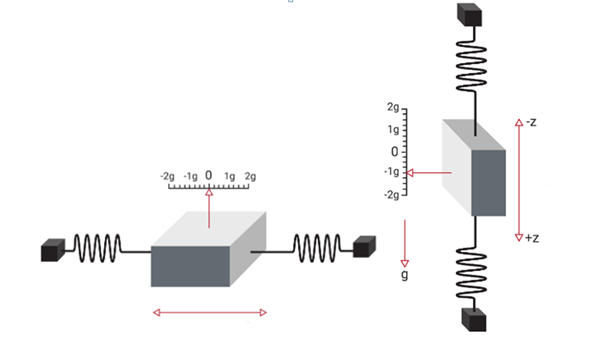
\includegraphics[width=\textwidth]{images/acce.png}
  \vspace*{-7mm}
  \caption{Nguyên lý cơ bản của cảm biến gia tốc}
  \label{acce}
\end{figure}

Như minh họa trong Hình~\ref{acce}, khi cảm biến gia tốc chịu tác động từ một
chuyển động, khối gia trọng (proof mass) sẽ dịch chuyển, làm lò xo kết nối bị
biến dạng.

Trong khuôn khổ luận văn này, tác giả tập trung tìm hiểu và ứng dụng cảm biến
gia tốc được chế tạo dựa trên công nghệ vi cơ điện tử (Micro-Electro-Mechanical
Systems – MEMS). Đây là một công nghệ tiên tiến cho phép tích hợp các thành
phần phần cứng siêu nhỏ và linh kiện điện tử ngay trên cùng một chip bán dẫn,
với kích thước cấu trúc có thể dưới 10 micromet. Một trong những ưu điểm nổi
bật của cảm biến gia tốc MEMS là khả năng tích hợp trực tiếp lên bo mạch in
(Printed Circuit Board – PCB), qua đó giảm thiểu thể tích chiếm dụng, tiết kiệm
chi phí sản xuất và đơn giản hóa thiết kế hệ thống nhúng. Nhờ đó, công nghệ này
đặc biệt phù hợp cho các ứng dụng trong thiết bị đeo cá nhân, điện thoại di
động, và các hệ thống theo dõi sức khỏe thế hệ mới.

Dựa trên nguyên lý chuyển đổi dao động cơ học thành tín hiệu điện, cảm biến gia
tốc MEMS được chia thành ba loại chính, mỗi loại ứng dụng một cơ chế vật lý
riêng biệt \cite{Acce, cambien}:

\begin{enumerate}
  \item \textbf{Cảm biến gia tốc kiểu điện dung (Capacitive Accelerometers)}:

        Đây là loại cảm biến phổ biến nhất trong các thiết bị điện tử tiêu dùng như điện thoại thông minh, vòng đeo tay sức khỏe và các hệ thống theo dõi chuyển động đeo được. Nguyên lý hoạt động của cảm biến dựa trên sự thay đổi điện dung giữa các bản cực trong cấu trúc tụ điện khi khối gia trọng (\textit{proof mass}) dịch chuyển dưới tác động của gia tốc.

        Khi có gia tốc tác động, khối lượng vi mô được treo bằng hệ lò xo vi cơ (MEMS
        spring system) sẽ dịch chuyển, làm thay đổi khoảng cách giữa các bản cực. Biến
        thiên điện dung này được ghi nhận thông qua mạch đo điện dung nhạy, sau đó được
        khuếch đại và chuyển đổi thành tín hiệu điện tỷ lệ với gia tốc. Ưu điểm chính
        bao gồm: độ nhạy cao ở vùng tần số thấp, kích thước nhỏ, tiêu thụ năng lượng
        thấp và khả năng tích hợp tốt vào các hệ thống nhúng. Loại cảm biến này đặc
        biệt phù hợp với các ứng dụng theo dõi tư thế và chuyển động chậm.

        \begin{figure}[H]
          \centering
          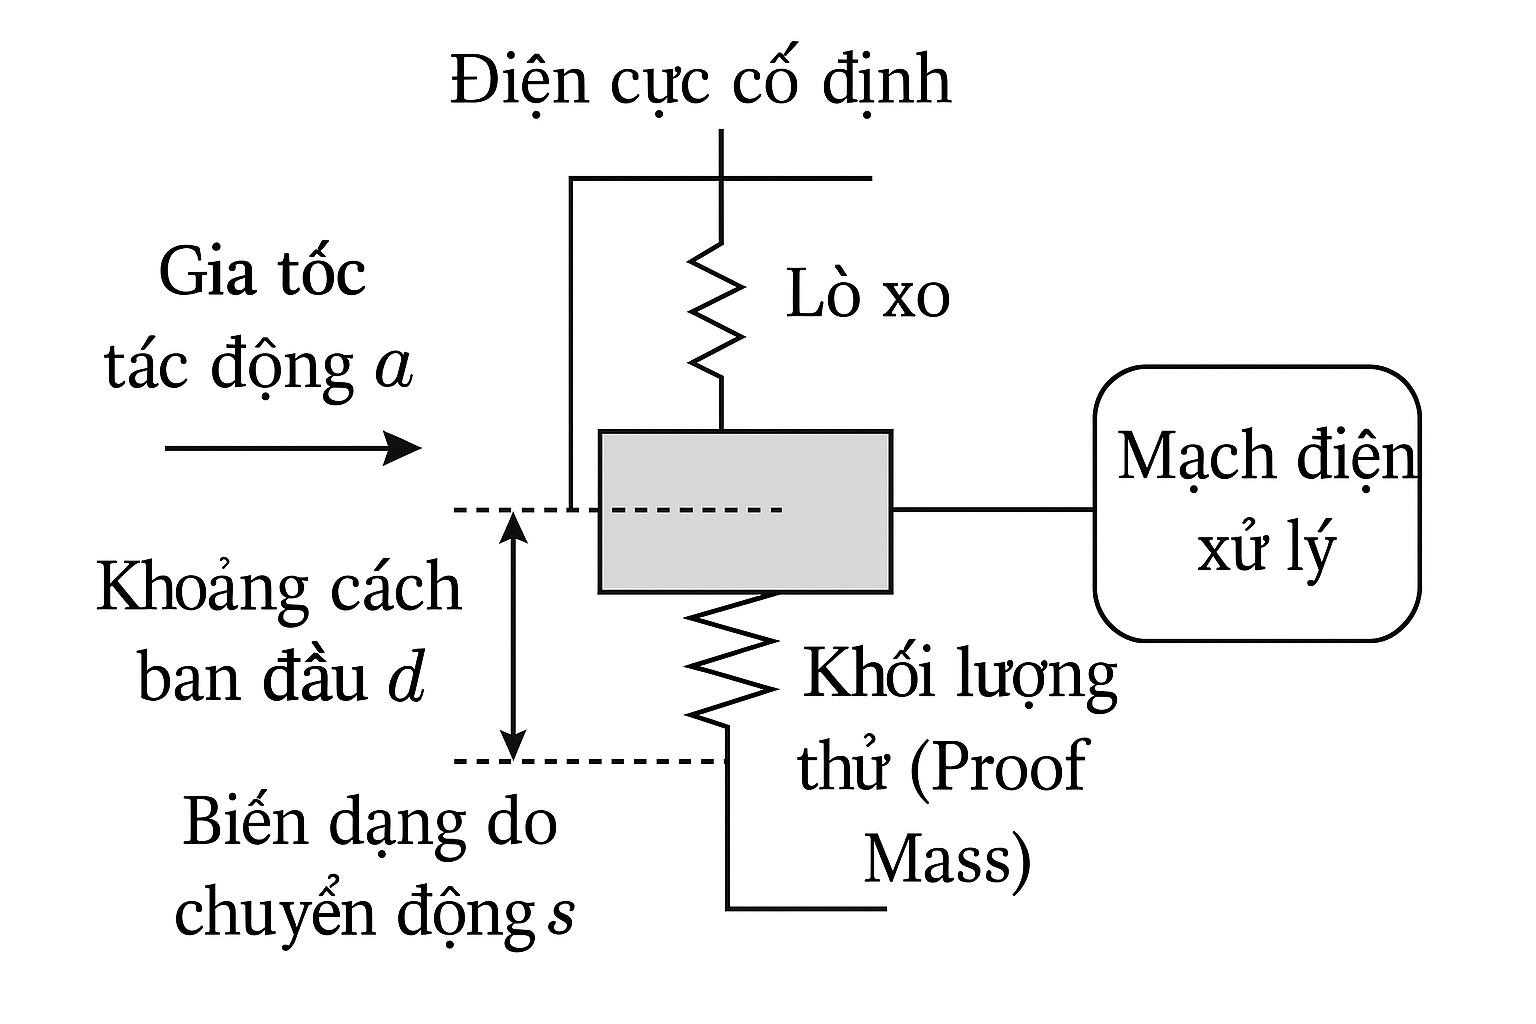
\includegraphics[width=0.7\textwidth]{images/diendung.png}
          \vspace*{-7mm}
          \caption{Cấu trúc cảm biến gia tốc điện dung}
          \label{acce_mems}
        \end{figure}

  \item \textbf{Cảm biến gia tốc kiểu áp điện trở (Piezoresistive Accelerometers)}:

        Loại cảm biến này hoạt động dựa trên hiện tượng thay đổi điện trở của vật liệu
        bán dẫn khi chịu ứng suất cơ học – còn gọi là hiệu ứng áp điện trở. Các phần tử
        cảm biến thường được gắn trực tiếp lên thanh dầm (cantilever) nối với khối gia
        trọng. Khi có gia tốc, sự biến dạng cơ học của thanh dầm làm thay đổi điện trở
        của phần tử cảm biến.

        Để tăng độ nhạy và khả năng khuếch đại tín hiệu, cấu trúc cảm biến thường được tích hợp trong mạch cầu Wheatstone, giúp tăng cường tỷ số tín hiệu trên nhiễu (Signal-to-Noise Ratio – SNR).

        \begin{figure}[H]
          \centering
          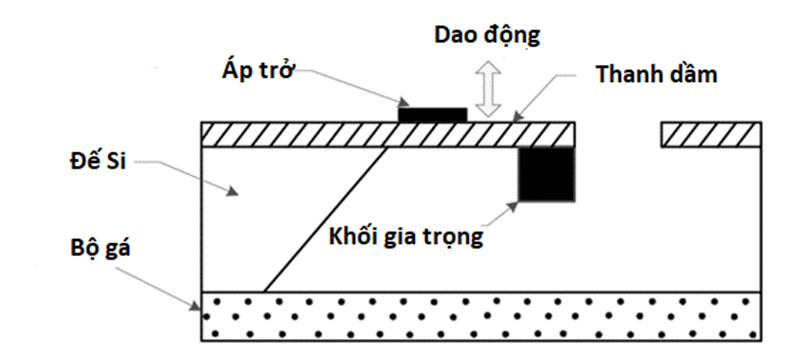
\includegraphics[width=\textwidth]{images/acce_aptro.png}
          \vspace*{-7mm}
          \caption{Cấu trúc cảm biến áp điện trở}
          \label{acce_aptro}
        \end{figure}

        Ưu điểm chính của cảm biến áp điện trở là khả năng hoạt động
        ổn định trong môi trường nhiệt độ cao hoặc điều kiện công nghiệp khắc nghiệt.
        Tuy nhiên, chúng tiêu thụ nhiều năng lượng hơn và kém nhạy hơn
        với chuyển động biên độ nhỏ, do đó ít phù hợp với các ứng dụng
        theo dõi sinh lý học dài hạn như tư thế ngủ.

  \item \textbf{Cảm biến gia tốc kiểu áp điện (Piezoelectric Accelerometers)}:

        Dựa trên hiệu ứng áp điện, cảm biến kiểu này sử dụng các vật liệu như thạch anh
        hoặc gốm sứ có khả năng tạo ra điện tích khi bị biến dạng (nén hoặc kéo). Lượng
        điện tích sinh ra tỉ lệ thuận với lực cơ học tác động lên cảm biến.

        \begin{figure}[H]
          \centering
          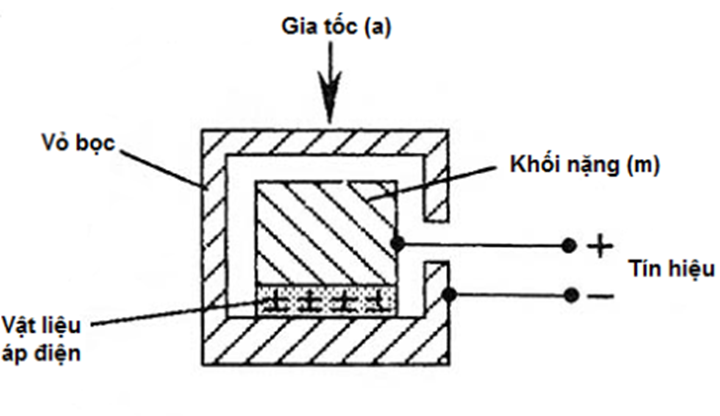
\includegraphics[width=\textwidth]{images/acce_apdien.png}
          \vspace*{-7mm}
          \caption{Cấu trúc cảm biến áp điện}
          \label{acce_apdien}
        \end{figure}

        Cảm biến kiểu áp điện có ưu điểm nổi bật là khối lượng nhẹ, tốc độ phản hồi
        nhanh, và dải tần hoạt động rất rộng (có thể lên tới hàng MHz). Chúng thường
        được ứng dụng trong đo rung động chính xác, giám sát kết cấu, và phân tích chấn
        động ngắn hạn trong môi trường khắc nghiệt.

        Tuy cảm biến áp điện có độ nhạy cao với rung động nhanh và tần số cao, nhưng
        chúng không phù hợp để đo gia tốc tĩnh hoặc chuyển động chậm kéo dài – vốn là
        đặc trưng của bài toán theo dõi tư thế ngủ. Nguyên nhân là vì cảm biến này
        không phản hồi với lực không đổi như trọng lực, do điện tích tạo ra bị rò dần
        theo thời gian. Bên cạnh đó, tín hiệu đầu ra có trở kháng rất cao, dễ suy hao,
        đòi hỏi bộ khuếch đại điện tích chuyên dụng, làm tăng độ phức tạp, kích thước
        và tiêu thụ năng lượng của hệ thống. Những yếu tố này khiến cảm biến áp điện
        không phù hợp để tích hợp vào thiết bị đeo cá nhân dùng trong theo dõi OSA tại
        nhà.
\end{enumerate}

Trong khuôn khổ luận văn này, cảm biến gia tốc MEMS kiểu điện dung được lựa
chọn làm phần tử cảm biến trung tâm cho hệ thống theo dõi tư thế ngủ kéo dài,
trên cơ sở đánh giá đa chiều cả về đặc trưng tín hiệu, yêu cầu hệ thống, lẫn
khả năng triển khai thực tế.

Thứ nhất, từ góc độ \textit{đặc trưng tín hiệu}, bài toán nhận diện tư thế ngủ
yêu cầu hệ thống có khả năng ghi nhận chính xác các chuyển động biên độ nhỏ,
xảy ra chậm rãi trong thời gian dài (ví dụ như quá trình xoay người khi ngủ
hoặc chuyển từ nằm ngửa sang nghiêng). Đây là điều kiện lý tưởng cho cảm biến
điện dung MEMS – vốn có độ nhạy cao trong vùng tần số thấp (DC đến vài chục
Hz), cho phép nhận diện rõ ràng sự thay đổi hướng trọng lực tác động lên trục
cảm biến. Không giống như cảm biến áp điện, vốn chỉ phản hồi với dao động nhanh
và không ghi nhận được trạng thái tĩnh, cảm biến điện dung cho phép theo dõi
liên tục tư thế cơ thể với độ ổn định tín hiệu cao, phù hợp với đặc điểm sinh
lý của giấc ngủ.

Thứ hai, về \textit{yêu cầu hệ thống}, thiết bị theo dõi tư thế ngủ tại nhà cần
đảm bảo ba yếu tố: (i) tiêu thụ năng lượng thấp để hoạt động xuyên đêm bằng
pin; (ii) kích thước nhỏ gọn để đeo thoải mái mà không ảnh hưởng đến giấc ngủ;
và (iii) khả năng tích hợp lên vi điều khiển nhúng (như dòng ARM Cortex-M) nhằm
xử lý tín hiệu tại chỗ mà không cần truyền tải liên tục về máy chủ. Cảm biến
điện dung MEMS đáp ứng hoàn toàn các yêu cầu này: tiêu thụ năng lượng ở mức vài
µA, kích thước thường chỉ vài mm$^2$, và tín hiệu đầu ra dạng điện áp hoặc giao
tiếp I\textsuperscript{2}C/SPI – thuận tiện cho việc kết nối với hệ thống nhúng
tiêu chuẩn.

Thứ ba, xét về \textit{tính khả thi triển khai}, cảm biến điện dung MEMS có chi
phí sản xuất và tích hợp thấp hơn rõ rệt so với các loại cảm biến dùng hiệu ứng
áp điện hoặc áp điện trở, vốn yêu cầu mạch xử lý tín hiệu chuyên biệt (như
khuếch đại điện tích hoặc cầu đo điện trở chính xác). Hơn nữa, loại cảm biến
này có độ phổ biến cao trong chuỗi cung ứng linh kiện, dễ dàng tìm thấy các
model tối ưu (như LIS3DH, ADXL345, MMA8451Q\ldots) với đầy đủ tài liệu kỹ
thuật, thư viện lập trình và driver mã nguồn mở – giúp rút ngắn thời gian phát
triển, tăng tính linh hoạt và khả năng tái sử dụng của hệ thống.

Cuối cùng, việc sử dụng cảm biến điện dung không chỉ đảm bảo độ chính xác đo
lường trong môi trường thử nghiệm mà còn mang lại độ tin cậy và tính thực tiễn
cao khi triển khai ở quy mô cộng đồng. Thiết kế hệ thống đơn giản, tiêu thụ
điện năng thấp, dễ chế tạo và mở rộng – đây là những yếu tố then chốt trong các
giải pháp y học số (digital health) hướng tới phòng ngừa sớm và giám sát cá
nhân hoá tại nhà.

\textbf{Tóm lại}, việc lựa chọn cảm biến điện dung MEMS không đơn thuần là một quyết định kỹ thuật thuần tuý, mà còn phản ánh một giải pháp có tính cân bằng giữa hiệu quả đo lường, khả năng tích hợp phần cứng, và chiến lược mở rộng ứng dụng lâm sàng theo hướng chi phí thấp. Đây là một trong những nguyên tắc then chốt trong xu hướng đổi mới công nghệ y tế cộng đồng hiện đại – nơi mà tính khả thi triển khai và khả năng mở rộng đóng vai trò không kém phần quan trọng so với độ chính xác kỹ thuật.

\vspace{1em}

Nhìn chung, việc chẩn đoán hội chứng ngưng thở khi ngủ – đặc biệt là thể ngưng
thở tắc nghẽn phụ thuộc tư thế (positional OSA – pOSA) – đòi hỏi một hệ thống
giám sát liên tục, có khả năng thu thập dữ liệu sinh lý trong thời gian dài,
nhận diện chính xác tư thế ngủ, và đưa ra cảnh báo kịp thời trong môi trường
sinh hoạt tự nhiên tại nhà. Những yêu cầu này không chỉ giới hạn ở độ chính xác
mô hình, mà còn mở rộng tới tiêu chí về tính gọn nhẹ, tiết kiệm năng lượng, và
dễ triển khai trên nền tảng vi điều khiển hoặc thiết bị đeo.

Trong bối cảnh đó, các mô hình học máy trở thành công cụ thiết yếu để khai thác
dữ liệu cảm biến. Chúng không chỉ cho phép phân loại tư thế với độ chính xác
cao mà còn mở rộng sang suy luận các chỉ số lâm sàng như AHI. Việc triển khai
trực tiếp trên vi điều khiển Cortex-M4 theo hướng TinyML đưa giải pháp từ phòng
thí nghiệm đến ứng dụng thực tiễn tại nhà, đánh dấu sự giao thoa giữa y học
giấc ngủ truyền thống và trí tuệ nhân tạo ứng dụng – một lĩnh vực đang phát
triển mạnh mẽ trong thập niên gần đây \cite{osa_sanchez2025}.

\subsection{Quy trình tổng quát trong hệ thống ứng dụng AI cho đánh
  giá OSA và phân loại tư thế ngủ}
\begin{table}[htbp]
  \centering
  \caption{Các bước chính trong hệ thống ứng dụng AI cho phân tích tư thế ngủ và hỗ trợ chẩn đoán OSA}
  \label{tab:pipeline_steps}
  \small
  \renewcommand{\arraystretch}{1.2}
  \begin{tabular}{|c|p{3.8cm}|p{9.2cm}|}
    \hline
    \textbf{STT} & \textbf{Giai đoạn}                                                             & \textbf{Mô tả tổng quát}                                                                                                                         \\
    \hline
    1            & \textbf{Thu thập tín hiệu} \newline (Data Acquisition)                         & Ghi nhận tín hiệu từ cảm biến như gia tốc ba trục, PPG, ECG hoặc áp lực. Thiết bị đeo nhỏ gọn, truyền dữ liệu qua BLE, tốc độ lấy mẫu 10–100 Hz. \\
    \hline
    2            & \textbf{Tiền xử lý tín hiệu} \newline (Preprocessing)                          & Lọc nhiễu (notch, bandpass), loại bỏ trôi nền, phân đoạn theo cửa sổ thời gian. Mục tiêu là làm sạch và ổn định dữ liệu đầu vào.                 \\
    \hline
    3            & \textbf{Trích xuất đặc trưng} \newline (Feature Extraction)                    & Tính toán các đặc trưng thời gian (mean, std, energy...) và tần số (FFT, wavelet), đại diện cho nội dung sinh lý trong từng đoạn tín hiệu.       \\
    \hline
    4            & \textbf{Lựa chọn và huấn luyện mô hình} \newline (Model Selection \& Training) & Lựa chọn thuật toán học máy (SVM, RF, LR, NN nhẹ) phù hợp với bài toán phân loại tư thế và/hoặc đánh giá OSA.                                    \\
    \hline
    5            & \textbf{Đánh giá hiệu năng} \newline (Evaluation)                              & Sử dụng các chỉ số đánh giá mô hình như Accuracy, Precision, Recall, F1-Score, AUC, confusion matrix.                                            \\
    \hline
    6            & \textbf{Tối ưu mô hình} \newline (Model Optimization)                          & Ứng dụng kỹ thuật pruning, quantization (8-bit) để giảm kích thước và độ phức tạp mô hình nhằm phục vụ triển khai biên.                          \\
    \hline
    7            & \textbf{Triển khai thực tế} \newline (Deployment)                              & Triển khai mô hình trên vi điều khiển (MCU) hỗ trợ TinyML, tích hợp trong thiết bị đeo nhằm theo dõi tư thế ngủ và ước lượng AHI tại nhà.        \\
    \hline
  \end{tabular}
\end{table}

Quy trình này có thể được điều chỉnh tùy theo loại tín hiệu đầu vào và mục tiêu
phân tích cụ thể (nhận diện tư thế, phát hiện ngưng thở, theo dõi nhịp
thở,...). Tuy nhiên, nguyên tắc cơ bản là đảm bảo tín hiệu đầu vào chất lượng
cao và mô hình đủ nhẹ để triển khai thực tế (xem
Bảng~\ref{tab:pipeline_steps}).

\textbf{Thu thập tín hiệu} là bước đầu tiên và đóng vai trò nền tảng
trong toàn bộ quy trình phân tích tư thế ngủ, chẩn đoán hội chứng ngưng
thở khi ngủ (OSA) bằng trí tuệ nhân tạo. Trong các hệ thống theo dõi tại
nhà (HST), quá trình này được thực hiện thông qua các thiết bị đeo hoặc
cảm biến gắn ngoài, với mục tiêu ghi nhận liên tục các tín hiệu sinh
lý phản ánh hoạt động hô hấp, tuần hoàn và chuyển động cơ thể trong
suốt giấc ngủ.
Tín hiệu được ghi nhận có thể bao gồm: gia tốc ba trục nhằm phát hiện
chuyển động và tư thế nằm; tín hiệu PPG để đo nhịp tim và độ bão hòa oxy;
tín hiệu ECG để đánh giá hoạt động điện tim; hoặc tín hiệu từ cảm biến hô
hấp, cảm biến áp lực gắn trên giường để xác định tư thế ngủ qua phân
bố trọng lực. Tuỳ vào mục tiêu nghiên cứu và cấu hình thiết bị, các tín
hiệu này được lấy mẫu với tần số phù hợp, thường dao động từ 10 Hz đến
500 Hz \cite{Sleep_Posture_Detection, Jeng, Zhang_osa, Ferrer_osa, Sang, osa_sanchez2025}.
Một trong những yêu cầu quan trọng của bước thu thập là đảm bảo tính
ổn định và chất lượng của dữ liệu. Các cảm biến cần được gắn chắc chắn
tại những vị trí tối ưu, chẳng hạn như vùng ngực, cổ tay hoặc hõm ức,
để giảm thiểu nhiễu do chuyển động và duy trì tiếp xúc ổn định trong
suốt quá trình theo dõi. Ngoài ra, hệ thống cũng cần đảm bảo khả năng
lưu trữ hoặc truyền dữ liệu hiệu quả thông qua các giao thức không dây
như Bluetooth Low Energy (BLE) hoặc Wi-Fi \cite{thuong_wear_paper, hst_wear_paper}.
Trong một số nghiên cứu gần đây, các hệ thống HST hiện đại đã sử dụng
vi điều khiển công suất thấp tích hợp cảm biến gia tốc, cho phép truyền
dữ liệu liên tục với mức tiêu thụ năng lượng tối ưu. Ví dụ, trong nghiên
cứu \cite{Sleep_Posture_Detection}, thiết bị dán cổ tích hợp cảm biến gia
tốc LIS2DH12 và vi điều khiển nRF5232 đã được sử dụng để thu tín hiệu ở
tần số 100 Hz và truyền không dây qua BLE, đảm bảo dữ liệu ổn định và
chính xác trong điều kiện thực tế tại nhà.

Chất lượng của dữ liệu thu được trong bước này ảnh hưởng trực tiếp đến hiệu quả
của toàn bộ hệ thống. Do đó, quá trình thu thập tín hiệu cần được thiết kế sao
cho vừa đáp ứng được yêu cầu về độ chính xác sinh lý, vừa đảm bảo tính khả thi
khi triển khai lâu dài trong môi trường ngoài lâm sàng. Tuy nhiên, trong nhiều
nghiên cứu hiện nay, cấu trúc phần mềm cho quá trình thu thập và lưu trữ dữ
liệu vẫn chưa được trình bày một cách đầy đủ và thống nhất. Các yếu tố như kiến
trúc hệ thống (ứng dụng di động, web, hay máy chủ trung tâm), giao thức truyền
thông (MQTT, HTTP), phương thức lưu trữ (cục bộ, cloud, hoặc cơ sở dữ liệu liên
kết), cũng như các vấn đề liên quan đến mã hóa – bảo mật dữ liệu sức khỏe – và
tuân thủ quy định của cơ quan chuyên môn (chuẩn HIPAA, GDPR, hoặc quy định y tế
quốc gia) thường chưa được đề cập rõ ràng. Những yếu tố này có thể ảnh hưởng
đến khả năng mở rộng, tích hợp, và ứng dụng thực tiễn của hệ thống trong môi
trường chăm sóc sức khỏe tại nhà.

\subsubsection{Tiền xử lý dữ liệu}

\textbf{Tiền xử lý dữ liệu} là một giai đoạn quan trọng nhằm cải thiện
chất lượng tín hiệu, chuẩn hóa định dạng đầu vào và đảm bảo tính đồng
nhất của dữ liệu trước khi đưa vào mô hình học máy. Các kỹ thuật tiền xử
lý phổ biến bao gồm lọc tín hiệu (filtering), nội suy (interpolation),
chuẩn hóa dữ liệu (normalization), phân đoạn tín hiệu (Segmentation – Epoch Creation).

\textbf{Lọc tín hiệu} là bước đầu tiên trong tiền xử lý nhằm loại bỏ nhiễu khỏi
các tín hiệu sinh lý như EEG, ECG, EMG, $\mathrm{SpO_2}$ và gia tốc.
Các loại nhiễu thường gặp bao gồm: nhiễu điện lưới (50–60 Hz),
chuyển động cơ thể (motion artifacts), nhiễu tần số cao và trôi đường
cơ sở (baseline drift) \cite{rossi2023sleep, sheta2021osa }.
Trong nghiên cứu của Sheta và cộng sự \cite{sheta2021osa}, tác giả đã sử
dụng bộ lọc notch IIR bậc hai nhằm loại bỏ nhiễu điện lưới 60~Hz khỏi
tín hiệu ECG — vốn là loại nhiễu phổ biến gây khó khăn cho việc phân
tích và trích xuất đặc trưng hình thái. Kết quả cho thấy tín hiệu sau
lọc cho chất lượng cao hơn đáng kể và cải thiện hiệu năng của các mô
hình học máy trong chẩn đoán OSA.
Các kỹ thuật lọc phổ biến bao gồm notch filter
(đặc biệt là IIR notch filter bậc hai) để loại bỏ nhiễu điện lưới,
bandpass filter để giữ lại dải tần sinh lý, và
các bộ lọc mượt như Butterworth bậc ba, median filter hoặc
moving average filter.
Đối với tín hiệu gia tốc, các bộ lọc cần đảm bảo vừa loại bỏ nhiễu vừa
bảo toàn các đặc trưng chuyển động. Trong đó, Kalman filter được sử dụng
rộng rãi để làm mượt chuỗi tín hiệu thời gian và giảm nhiễu ngẫu nhiên,
còn total variation filter được đánh giá cao trong việc bảo toàn biên
chuyển động rõ nét \cite{kalman, sun2017sleepmonitor}.
Việc lựa chọn bộ lọc phù hợp cần dựa trên đặc điểm của từng loại
tín hiệu và mục tiêu phân tích cụ thể.

\textbf{Nội suy}
là bước cần thiết để chuẩn hóa chuỗi thời gian. Các phương pháp như
cubic spline, piecewise cubic Hermite (PCHIP) hay linear interpolation
thường được áp dụng để điều chỉnh các chuỗi dữ liệu về cùng tần số chuẩn,
đảm bảo đầu vào đồng bộ cho mô hình học máy hoặc mạng nơ-ron.
Ngoài ra, đối với các chuỗi tín hiệu rời rạc như nhịp RR từ ECG
hoặc các chuỗi $\mathrm{SpO_2}$ có thể bị gián đoạn hoặc mất mẫu,
kỹ thuật nội suy còn đóng vai trò quan trọng trong việc làm đầy các
giá trị bị thiếu (missing/null values) và tái cấu trúc tín hiệu thành
chuỗi liên tục, giúp mô hình học được đặc trưng đầy đủ hơn từ
dữ liệu \cite{zou2024mbtcn}.
Trong nghiên cứu \cite{olsen2024transfer},
cả hai tín hiệu gia tốc (ACC) và xung quang học (PPG)
đều được nội suy để tạo thành chuỗi thời gian đồng nhất với
tần số lấy mẫu 32 Hz.
Đối với các tín hiệu có tần số cao hơn 32 Hz,
một bộ lọc thông thấp (lowpass filter) được áp dụng trước khi giảm
tần số (down-sampling) nhằm hạn chế hiện tượng aliasing.
Ngược lại, các tín hiệu có tần số lấy mẫu thấp hơn 32 Hz được
nội suy bằng phương pháp đa thức Hermite từng đoạn
(PCHIP – Piecewise Cubic Hermite Interpolation Polynomial)
để khớp với tần số mong muốn.

\textbf{Chuẩn hóa dữ liệu}  giúp đưa các đặc trưng đầu vào về cùng một miền giá trị,
tránh hiện tượng các đặc trưng có biên độ lớn chi phối quá trình học.
Một số phương pháp phổ biến bao gồm: Z-score normalization
(chuẩn hóa về trung bình 0 và độ lệch chuẩn 1),
min-max scaling (đưa về khoảng [0,1]), và robust scaling
(dựa trên trung vị và IQR, phù hợp với dữ liệu có nhiễu hoặc ngoại lệ).
Trong các nghiên cứu về OSA, chuẩn hóa đã được áp dụng cho nhiều
loại tín hiệu như $\mathrm{SpO_2}$, PPG và gia tốc, giúp tăng độ ổn định
mô hình và cải thiện tốc độ hội tụ khi huấn luyện mạng nơ-ron
\cite{Sleep_Posture_Detection, Vu2025SleepPosition, rossi2023sleep}.

\textbf{Phân đoạn tín hiệu} là một bước thiết yếu trong xử lý tín
hiệu sinh lý, đặc biệt trong các hệ thống theo dõi vị trí giấc ngủ và phát
hiện ngưng thở khi ngủ (OSA). Mục tiêu của bước này là chia chuỗi dữ
liệu liên tục thành các đoạn thời gian ngắn cố định (epoch),
giúp mô hình học máy nhận diện hiệu quả các đặc trưng biến đổi theo
thời gian. Thời lượng epoch thường phụ thuộc vào loại tín hiệu và
mục tiêu phân tích: 30 giây cho EEG, 60 giây cho ECG và $\mathrm{SpO_2}$,
5 phút cho HRV, hoặc các cửa sổ trượt ngắn để phát hiện sự kiện ngắn hạn.
Trong một số trường hợp, việc phân đoạn còn dựa vào các đặc điểm sinh lý
như đỉnh sóng R trong ECG. Sau khi phân đoạn, các bước tiền xử lý như lọc nhiễu,
chuẩn hóa hoặc làm mượt được áp dụng trong từng đoạn để nâng cao c
hất lượng dữ liệu đầu vào cho mô hình học máy
\cite{Sleep_Posture_Detection, Vu2025SleepPosition, HOANG2025116309, zou2024mbtcn, osa_sanchez2025}.

Tóm lại, tiền xử lý tín hiệu không chỉ giúp nâng cao chất lượng dữ liệu mà còn
đảm bảo tính nhất quán đầu vào cho hệ thống học máy. Việc lựa chọn kỹ thuật
tiền xử lý cần phù hợp với đặc điểm của từng loại tín hiệu và mục tiêu phân
tích cụ thể.

\subsubsection{Trích xuất đặc trưng}
\textbf{Trích xuất đặc trưng} là một bước quan trọng nhằm biến đổi dữ liệu cảm biến
thô thành tập hợp các đặc trưng có ý nghĩa, phản ánh các mẫu hình sinh lý
liên quan đến mục đích của nghiên cứu. Quá trình này giúp làm nổi bật
những thông tin cốt lõi từ tín hiệu sinh học như ECG, PPG,
$\mathrm{SpO_2}$, gia tốc hay tín hiệu hô hấp, phục vụ cho các mô hình
học máy trong việc phân loại tư thế ngủ hoặc phát hiện hội chứng ngưng
thở khi ngủ (OSA) \cite{hstSurvey, HOANG2025116309, Channa_osa, Uday, Sang}.
Các đặc trưng thường được sử dụng bao gồm biến thiên
nhịp tim (HRV), khoảng RR, biên độ sóng R từ tín hiệu ECG; các chỉ số
thống kê, tần số và entropy từ tín hiệu $\mathrm{SpO_2}$; hoặc các đặc
trưng phi tuyến và miền tần số như năng lượng phổ, thông số Hjorth từ EEG.
Ngoài ra, các đặc trưng từ tín hiệu PPG và gia tốc như entropy, phương sai
hoặc số lượng chuyển động cũng đóng vai trò quan trọng trong việc phản ánh
mức độ rối loạn hô hấp trong giấc ngủ. Ngoài các đặc trưng truyền thống
trong miền thời gian và tần số, các đặc trưng hỗn hợp như biến đổi
wavelet đã chứng minh vai trò đặc biệt quan trọng trong việc mô tả
tín hiệu sinh lý một cách toàn diện hơn. Cụ thể, biến đổi wavelet
cho phép phân tích tín hiệu ở nhiều thang thời gian khác nhau, đồng thời
bảo toàn được cả thông tin về thời điểm và cấu trúc tần số của tín hiệu.
Điều này đặc biệt hữu ích trong bối cảnh tín hiệu sinh lý thường không
ổn định (non-stationary), như tín hiệu ECG, PPG hoặc tín hiệu gia tốc
trong quá trình theo dõi tư thế ngủ. Các hệ số wavelet thu được từ tín
hiệu gốc có thể phản ánh rõ ràng sự thay đổi chu kỳ hô hấp, chuyển động
cơ thể, cũng như các đặc điểm bất thường liên quan đến cơn ngưng thở khi
ngủ. Nhờ đó, việc trích xuất đặc trưng wavelet đóng góp quan trọng vào
hiệu suất của các mô hình phân loại tư thế ngủ và phát hiện OSA \cite{Sleep_Posture_Detection}.

\textbf{Gán nhãn (labeling)}
được thực hiện nhằm liên kết các phân đoạn tín hiệu với nhãn sự kiện
hô hấp tương ứng như “Apnea”, “Hypopnea”, hoặc phân mức độ nặng của OSA
như “Mild”, “Moderate”, “Severe”. Một số nghiên cứu còn mở rộng sang
các nhãn liên quan đến chất lượng tín hiệu (“Good” vs. “Poor”),
kiểu hô hấp (“Bình thường”, “Bất thường”), các nhãn liên quan đến tư thế ngủ.
Việc gán nhãn đúng đắn giúp huấn luyện mô hình
AI chính xác và đánh giá mức độ nghiêm trọng của OSA một cách hiệu quả.
Tùy theo thiết kế nghiên cứu, nhãn có thể được gán thủ công dựa trên
chuyên gia hoặc tự động đồng bộ với thiết bị tham chiếu như
camera, hệ thống PSG.

\textbf{Phát hiện đỉnh (peak detection)} là kỹ thuật thường được áp dụng
để trích xuất thông tin từ tín hiệu dạng sóng, đặc biệt là ECG và PPG.
Trong các nghiên cứu về OSA, đỉnh sóng R từ ECG thường được xác định
để tính toán HRV, sử dụng các thuật toán như Pan–Tompkins, Hamilton
hoặc ngưỡng thích nghi (adaptive threshold) \cite{osa_sanchez2025}. Với tín hiệu PPG,
đỉnh tâm thu được phát hiện thông qua các thuật toán lặp hoặc
wavelet nhị phân để xác định các khoảng thời gian giữa hai đỉnh
(peak-to-peak intervals). Kỹ thuật này giúp nâng cao độ chính xác
trong việc phát hiện các thay đổi sinh lý, góp phần cải thiện năng
lực chẩn đoán tự động OSA trong các hệ thống ứng dụng trí tuệ nhân tạo.

\subsubsection{Lựa chọn và huấn luyện mô hình}
Các kỹ thuật học máy và kiến trúc mạng nơ-ron nhân tạo đã được ứng dụng hiệu
quả trong các bài toán phân loại tư thế ngủ và chẩn đoán hội chứng ngưng thở
khi ngủ (OSA). Học máy (Machine Learning – ML) cung cấp một tập hợp đa dạng các
thuật toán cho phép khai thác mẫu hình từ dữ liệu cảm biến, hỗ trợ phát hiện
những thay đổi trong tư thế cơ thể và các rối loạn hô hấp liên quan đến giấc
ngủ. Trong khi đó, mạng nơ-ron nhân tạo (Artificial Neural Networks – ANN), đặc
biệt là các kiến trúc sâu như CNN, LSTM hoặc hybrid CNN-LSTM, thể hiện ưu thế
trong việc xử lý tín hiệu sinh lý phi tuyến, phức tạp, có độ biến thiên cao
theo thời gian như ECG, $\mathrm{SpO_2}$ hay tín hiệu gia tốc ba trục.

Trong số các \textbf{thuật toán học máy truyền thống} được sử dụng phổ biến,
Random Forest (RF) \cite{genuer2020random} nổi bật nhờ khả năng kháng chống lại
quá khớp và độ chính xác cao. Trong nghiên cứu \cite{wang2023ml_wearable}, Wang
và cộng sự đã ứng dụng RF để phân loại các trường hợp ngưng thở khi ngủ, đạt độ
chính xác 93.88\%, độ nhạy 89.93\% và độ đặc hiệu 91.8\%. Một nghiên cứu khác
\cite{yeo2022respiratory}, Yeo và cộng sự sử dụng RF cho nhiệm vụ phân loại sự
kiện hô hấp, thu được độ chính xác 83\%, độ nhạy 99\% và F1-score 81\%. Mặc dù
có sự khác biệt về nguồn dữ liệu và phương pháp trích chọn đặc trưng, RF vẫn
cho thấy hiệu quả vượt trội khi so sánh với các thuật toán khác như SVM, LDA
hay QDA \cite{wang2023ml_wearable}, \cite{yeo2022respiratory},
\cite{parbat2024multiscale}.

Bên cạnh đó, thuật toán SVM \cite{cortes1995svm} cũng đã được áp dụng nhằm xác
định siêu phẳng tối ưu để phân loại các nhóm trong không gian đặc trưng. Trong
nghiên cứu \cite{wang2023ml_wearable}, Wang cũng sử dụng thêm mô hình SVM và
đạt độ chính xác 88,28\%, độ đặc hiệu 91,69\% và độ nhạy 83,94\%, cho thấy hiệu
quả cao trong phát hiện ngưng thở khi ngủ, dù mô hình Random Forest thường có
kết quả cao hơn. Ở nghiên cứu \cite{yeo2022respiratory}, SVM đạt độ chính xác
83\% và hệ số Cohen’s kappa 0,53 trong phân loại sự kiện hô hấp theo từng phút.
Trong \cite{parbat2024multiscale}, SVM được huấn luyện trên tín hiệu ECG một
kênh, đạt độ chính xác 69,13\%, góp phần cải thiện hiệu suất của hệ thống phân
loại khi tích hợp trong mô hình tổ hợp. Những kết quả này cho thấy SVM vẫn là
một phương pháp có giá trị trong ứng dụng học máy cho chẩn đoán ngưng thở khi
ngủ.

K-Nearest Neighbors (KNN) \cite{cunningham2007knn} là một thuật toán khác cũng
thường xuyên được áp dụng trong các nghiên cứu về phát hiện ngưng thở khi ngủ
\cite{wang2023ml_wearable}, \cite{jeon2020realtime}. Dựa trên nguyên lý đo độ
tương đồng trong không gian đặc trưng, KNN phân loại một điểm dữ liệu mới dựa
trên nhãn của các điểm lân cận gần nhất. Wang và cộng sự đã dùng mô hình KNN xử
lý tín hiệu quang học PPG và đạt độ chính xác 85.06\%, với độ đặc hiệu 86.11\%
và độ nhạy 83.72\% \cite{wang2023ml_wearable}. Trong khi đó, nghiên cứu
\cite{jeon2020realtime} báo cáo hiệu quả vượt trội hơn với accuracy lên đến
95\%, đồng thời vẫn đảm bảo thời gian thực thi đáp ứng yêu cầu hệ thống. Thành
công này được cho là đến từ khả năng đo lường chính xác độ tương đồng giữa dữ
liệu quan sát và dữ liệu đã học, giúp mô hình KNN đưa ra dự đoán phù hợp với
mức độ nghiêm trọng của OSA.

Bên cạnh các thuật toán truyền thống, mô hình XGBoost \cite{chen2016xgboost}
cũng được đưa vào thử nghiệm trong nghiên cứu \cite{wang2023ml_wearable} nhằm
đánh giá khả năng phân loại các mức độ ngưng thở khi ngủ. Là một biến thể của
thuật toán boosting, XGBoost được thiết kế tối ưu cho hiệu suất tính toán và có
khả năng xử lý hiệu quả cả bài toán hồi quy và phân loại. Kết quả cho thấy
XGBoost đạt độ chính xác 82.05\%, độ đặc hiệu 84.91\% và độ nhạy 78.42\%, cho
thấy tiềm năng lớn của mô hình này trong ứng dụng lâm sàng, đặc biệt trong các
hệ thống đòi hỏi cân bằng giữa độ chính xác và tốc độ huấn luyện. Trong nghiên
cứu \cite{yeo2022respiratory}, thuật toán Linear Discriminant Analysis (LDA)
\cite{tharwat2017lda} được đánh giá là một phương pháp quan trọng. LDA sử dụng
trung bình và ma trận hiệp phương sai của từng lớp để xác định ranh giới quyết
định tối ưu, nhằm tối đa hóa sự phân biệt giữa các lớp và giảm thiểu phương sai
nội bộ. Trong bối cảnh nghiên cứu, LDA cho thấy hiệu quả vượt trội trong phát
hiện sự kiện hô hấp với độ chính xác 81\%, độ nhạy 88\%, độ đặc hiệu 79\% và
điểm F1 đạt 81\%.

\textbf{Học sâu (Deep learning - DL)}là một lĩnh vực thuộc học máy
tập trung vào việc khai thác các mạng nơ-ron nhân tạo nhiều lớp để
trích xuất đặc trưng và mô hình hóa dữ liệu phức tạp. Các mô hình học
sâu đã chứng minh hiệu quả trong việc phát hiện tư thế ngủ, đánh giá tình trạng OSA.
Học sâu cho phép phân tích các tín hiệu sinh lý không tuyến tính,
có nhiễu và mang tính thời gian, chẳng hạn như tín hiệu PPG, ECG,
SpO\textsubscript{2} và gia tốc kế.

Khác với các mô hình học máy truyền thống vốn đòi hỏi kỹ thuật trích xuất đặc
trưng thủ công, các mạng học sâu có khả năng tự động học các đặc trưng biểu
diễn từ dữ liệu đầu vào thô thông qua quá trình huấn luyện. Điều này đặc biệt
hữu ích trong phát hiện hội chứng ngưng thở khi ngủ (OSA – \textit{Obstructive
  Sleep Apnea}), nơi tín hiệu thu nhận từ thiết bị đeo thường biến thiên theo tư
thế, giai đoạn ngủ và tình trạng sinh lý của từng bệnh nhân.

Trong các ứng dụng chẩn đoán OSA, nhiều kiến trúc học sâu đã được đề xuất và
triển khai, bao gồm mạng nơ-ron tích chập (Convolutional Neural Networks –
CNN), mạng nơ-ron hồi tiếp (Recurrent Neural Networks – RNN) với các biến thể
như LSTM (Long Short-Term Memory) và GRU (Gated Recurrent Unit), mạng nơ-ron
truyền thẳng (Feedforward Neural Networks – FNN), và mạng perceptron đa tầng
(Multilayer Perceptron – MLP). Ngoài ra, các mô hình học chuyển tiếp (Transfer
Learning) sử dụng các kiến trúc sâu như ResNet và ResNeXt cũng được chứng minh
mang lại hiệu quả cao trong bối cảnh dữ liệu hạn chế \cite{osa_sanchez2025,
  wang2023ml_wearable, rossi2023sleep, olsen2024transfer}. Gần đây, các mô hình
kết hợp giữa học sâu và phương pháp phân cụm phân cấp (Hierarchical Deep
Clustering – HDC) cũng được áp dụng nhằm giảm chi phí tính toán và mở rộng khả
năng triển khai trên các thiết bị vi xử lý nhúng.

Trong \cite{rossi2023sleep}, Rossi và cộng sự đã phát triển một mô hình mạng
nơ-ron sâu (DNN) được phát triển để xử lý tín hiệu siêu âm thu từ cảm biến đeo
ngực, theo hướng kết hợp đa cảm biến. Mô hình được thiết kế cho bài toán phân
loại ba chiều: chất lượng tín hiệu, các mẫu hô hấp và các mẫu giấc ngủ. Mô hình
đạt độ chính xác 96\% trong phân biệt tín hiệu nhiễu và bình thường, với độ
chính xác cao hơn trong dự đoán mẫu hô hấp (0.93) so với mẫu giấc ngủ (0.76).
Trong \cite{olsen2024transfer}, một mạng nơ-ron tích chập sâu (CNN) được triển
khai nhằm phân loại các giai đoạn ngủ và phát hiện ngưng thở khi ngủ từ thiết
bị CST (consumer sleep technologies) đeo tay, sử dụng tín hiệu từ cảm biến gia
tốc và PPG. Mô hình gồm hai luồng xử lý riêng biệt, và kết quả cho thấy hiệu
suất được cải thiện khi sử dụng dữ liệu thô, đặc biệt trong phát hiện sự kiện
apnea trong giấc ngủ REM. Ji et al và cộng sự triển khai mô hình Long
Short-Term Memory (LSTM) – một dạng mạng nơ-ron hồi tiếp (RNN) – nhằm phân tích
chuỗi tín hiệu sinh lý phục vụ phát hiện hội chứng ngưng thở – giảm thở khi ngủ
(SAHS) \cite{ji2022airline}. Mô hình gồm ba lớp lặp LSTM kết hợp với bốn lớp
kết nối đầy đủ, có số nút lần lượt là 128, 64, 32 và 1. Kết quả cho thấy mô
hình đạt độ chính xác trung bình từ 84–85\%, khẳng định tính hiệu quả của kiến
trúc LSTM trong việc nhận dạng các đặc trưng liên quan từ dữ liệu tuần tự. Tổng
thể, các mô hình học sâu như CNN, LSTM và các biến thể kết hợp đã chứng minh
hiệu quả vượt trội trong việc phát hiện OSA từ các tín hiệu sinh lý đa dạng.
Tuy nhiên, thách thức về chi phí tính toán, dung lượng bộ nhớ và khả năng triển
khai thực tế trên thiết bị đeo yêu cầu các hướng nghiên cứu tối ưu hóa mô hình
và giảm độ phức tạp.

Tập trung vào mục tiêu phát hiện các hoạt động thường ngày và tư thế ngủ của
con người, rất nhiều nghiên cứu gần đây đã ứng dụng các phương pháp học máy và
trí tuệ nhân tạo để xây dựng hệ thống nhận dạng từ dữ liệu cảm biến đeo được.
\textit{Bảng \ref{tab:sleepml}} dưới đây tổng hợp một số nghiên cứu tiêu biểu
trong lĩnh vực này, bao gồm cả các mô hình học máy truyền thống (như cây quyết
định, KNN, SVM) và các phương pháp học sâu (CNN, LSTM). Các hệ thống được triển
khai với mục đích phân loại tư thế ngủ hoặc hoạt động thể chất, sử dụng nhiều
loại dữ liệu cảm biến khác nhau như gia tốc ba trục, tín hiệu quang học (PPG)
hoặc đặc trưng miền thời gian. Nhiều nghiên cứu cũng đã chú trọng đến việc
triển khai mô hình trên thiết bị nhúng (on-chip), nhằm hướng đến khả năng theo
dõi tại nhà trong thời gian thực với chi phí và mức tiêu thụ năng lượng thấp.

Sự phát triển nhanh chóng của trí tuệ nhân tạo (AI) trong lĩnh vực y học đã mở
ra nhiều hướng tiếp cận mới trong việc đánh giá tư thế ngủ và chẩn đoán OSA.
Các hệ thống AI đang dần chứng minh hiệu quả vượt trội trong việc xử lý dữ liệu
cảm biến lớn và phức tạp, từ đó cung cấp các phân tích chính xác về hành vi
giấc ngủ của bệnh nhân. Các mô hình học máy được huấn luyện trên tập dữ liệu
cảm biến từ accelerometer, gyroscope hoặc thiết bị đeo thông minh có thể tự
động phân loại các tư thế ngủ theo thời gian thực, với độ chính xác lên đến
trên 90\% trong nhiều nghiên cứu gần đây
\cite{Sleep_Posture_Detection}\cite{Vu2025SleepPosition}\cite{HOANG2025116309}.

\textbf{Tiny Machine Learning (TinyML)} là lĩnh vực nghiên cứu và ứng dụng các
mô hình học máy có kích thước nhỏ gọn, tiêu thụ năng lượng thấp,
được triển khai trực tiếp trên các thiết bị nhúng như vi điều khiển
(microcontrollers – MCU) hoặc thiết bị đeo (wearables) \cite{ray2021tinyml}.
Không giống như các mô hình học máy truyền thống thường yêu cầu nền
tảng phần cứng mạnh và tính toán trên cloud, TinyML cho phép xử lý dữ
liệu tại chỗ (on-device inference) mà không cần kết nối internet,
nhờ đó nâng cao tính riêng tư, độ phản hồi thời gian thực và khả năng
hoạt động ngoại tuyến.

\begin{table}[htbp]
  \centering
  \caption{Hiệu quả mô hình học máy và khả năng triển khai biên trong nhận diện tư thế ngủ}
  \label{tab:sleepml}
  \small
  \renewcommand{\arraystretch}{1.2}
  \resizebox{\textwidth}{!}{%
    \begin{tabular}{|c|p{2.2cm}|p{2.2cm}|p{2.7cm}|p{3.3cm}|c|c|p{1.2cm}|}
      \hline
      \textbf{Tài liệu}     & \textbf{Dữ liệu}      & \textbf{Nhiệm vụ}    & \textbf{Đặc trưng}            & \textbf{Mô hình}              & \textbf{Độ chính xác} & \textbf{Phần mềm} & \textbf{On-chip} \\
      \hline
      \cite{abdulsadig2023} & 18 đối tượng          & Tư thế ngủ           & 12 đặc trưng miền thời gian   & DT, Extra-Trees, LSTM-NN      & $>$98\%               & NM                & Có               \\
      \cite{Jeng}           & Không nêu             & Tư thế ngủ           & NM                            & RF, SVM                       & 85\%                  & Có                & Không            \\
      \cite{vu2023}         & 561.859 mẫu           & Tư thế ngủ           & NM                            & LSTM\_sq, CNN, MLP, LSTM\_con & $>$99\%               & Không             & Không            \\
      \cite{kwasnicki2018}  & 16 đối tượng          & Tư thế ngủ           & Trung bình, 3 trục            & Ngưỡng cố định                & 99.5\%                & Không             & Không            \\
      \cite{elnaggar2023}   & 5 đối tượng           & Tư thế ngủ           & NM                            & Ngưỡng cố định                & $>$99.2\%             & Không             & Không            \\
      \cite{gomes2021}      & 8 đối tượng           & Hoạt động người dùng & Trung bình, Độ lệch chuẩn (6) & KNN, RF, SVM                  & 97\%                  & Không             & Không            \\
      \cite{dao2022}        & Public + 20 private   & Hoạt động người dùng & 31 đặc trưng miền thời gian   & RF                            & 97\%                  & Có                & Không            \\
      \cite{souza2017}      & 10 đối tượng (public) & Hoạt động người dùng & 11 đặc trưng miền thời gian   & KNN, NB, SVM, CTree, RF       & 98\%                  & Không             & Không            \\
      \hline
      \multicolumn{8}{l}{\footnotesize NM = Không đề cập; DT = Decision Tree; CNN = Convolutional Neural Network; MLP = Multilayer Perceptron;}                                                           \\
      \multicolumn{8}{l}{\footnotesize LSTM = Long Short-Term Memory; RF = Random Forest; SVM = Support Vector Machine; NB = Naive Bayes; CTree = Conditional Inference Tree.}
    \end{tabular}
  }
\end{table}

Trong lĩnh vực chăm sóc sức khỏe, công nghệ \textbf{TinyML} (Tiny Machine
Learning) ngày càng được ứng dụng rộng rãi để phân tích các tín hiệu sinh lý
như nhịp tim, nhịp thở, chuyển động và tư thế ngủ. Với ưu điểm tiêu thụ năng
lượng thấp, chi phí triển khai rẻ và khả năng vận hành lâu dài trên phần cứng
hạn chế, các mô hình TinyML đặc biệt phù hợp cho các hệ thống theo dõi y tế tại
nhà, chẳng hạn như phát hiện hội chứng ngưng thở khi ngủ (OSA) bằng thiết bị
đeo không xâm lấn. Các thuật toán thường được sử dụng trong TinyML bao gồm các
biến thể nhẹ và được đơn giản hóa từ các mô hình học sâu như
\textit{Convolutional Neural Networks (CNN)}, \textit{Long Short-Term Memory
  (LSTM)}, cùng với các mô hình cây quyết định gọn nhẹ như \textit{Decision
  Tree}, \textit{Random Forest} hoặc \textit{Gradient Boosting}, vốn đã được tối
ưu hoá cho việc hoạt động trên nền tảng vi điều khiển có giới hạn tài nguyên
(MCU).

Dữ liệu trong Bảng~\ref{tab:sleepml} cho thấy sự đa dạng trong cách tiếp cận
bài toán nhận diện tư thế ngủ và hoạt động người dùng. Hầu hết các nghiên cứu
đạt độ chính xác cao (trên 95\%), ngay cả khi sử dụng các thuật toán đơn giản
như ngưỡng cố định hoặc mô hình học máy cổ điển như KNN, SVM và RF. Tuy nhiên,
một điểm đáng lưu ý là chỉ duy nhất nghiên cứu của Abdulsadig và cộng sự
\cite{abdulsadig2023} thực sự được triển khai trên phần cứng nhúng (on-chip),
chứng tỏ tính khả thi trong môi trường tài nguyên hạn chế. Các nghiên cứu còn
lại chủ yếu dừng ở mức mô phỏng phần mềm hoặc chạy trên máy tính hiệu năng cao,
chưa đáp ứng được yêu cầu triển khai thực tế trong các thiết bị đeo.

Đi sâu hơn, nhóm mô hình học sâu như CNN, LSTM hoặc kết hợp nhiều lớp
(LSTM\_sq, LSTM\_con, MLP) tuy đạt độ chính xác vượt trội (trên 99\%) như trong nghiên cứu của Vu et al. \cite{vu2023}, nhưng đều chưa tích hợp trực tiếp lên vi điều khiển do dung lượng bộ nhớ lớn và nhu cầu tính toán cao. Điều này đặt ra thách thức cho việc ứng dụng chúng trong môi trường thực tế như giấc ngủ tại nhà, nơi mà năng lượng, khả năng lưu trữ và kết nối đều bị hạn chế.

Ở chiều ngược lại, các mô hình đơn giản hơn như Decision Tree,
Random Forest hay ngưỡng cố định cho thấy hiệu quả không hề thua
kém khi được khai thác đúng đặc trưng.
Đặc biệt, việc sử dụng các đặc trưng miền thời gian
(mean, std, energy, entropy) — vốn dễ tính toán và
không cần FFT — giúp giảm đáng kể độ phức tạp tính toán.
Điều này rất phù hợp với triết lý thiết kế của TinyML:
đơn giản, hiệu quả và khả thi khi triển khai thực
tế trên các nền tảng hạn chế như MCU.

Một điểm sáng là khả năng cải thiện hiệu năng của mô hình bằng cách lựa chọn
đặc trưng phù hợp với tín hiệu đầu vào. Ví dụ, các đặc trưng trung bình và
phương sai theo trục trong các nghiên cứu \cite{gomes2021}, \cite{souza2017} đủ
mạnh để phân biệt các tư thế ngủ hoặc hoạt động cơ bản, mà không cần tới biểu
diễn phức tạp trong miền tần số hay wavelet.

Nhờ sự phát triển của các nền tảng hỗ trợ triển khai mô hình học máy như
\textbf{TensorFlow Lite for Microcontrollers}, \textbf{Edge Impulse}, và
\textbf{TinyML EON Compiler}, việc huấn luyện, chuyển đổi và triển khai các mô
hình chỉ yêu cầu vài kilobyte bộ nhớ đã trở nên khả thi. Điều này mở ra hướng
tiếp cận mới trong chẩn đoán y tế cá nhân hóa, thông qua thiết bị đeo thông
minh hoạt động liên tục tại nhà.

Một điểm mạnh nổi bật của các mô hình AI triển khai trên nền TinyML là khả năng
học và tự hiệu chỉnh theo dữ liệu thực tế. Nhờ vậy, hệ thống có thể phân biệt
hiệu quả giữa các tư thế ngủ cơ bản — nghiêng trái, nghiêng phải, nằm ngửa, và
nằm sấp — ngay cả khi có những sai lệch nhỏ về góc đặt thiết bị hoặc chuyển
động cơ thể không mong muốn. Hơn nữa, AI còn cho phép tích hợp dữ liệu tư thế
với các thông số sinh lý khác như nhịp tim, nhịp thở, độ bão hòa oxy máu
(SpO$_2$), và âm thanh để xây dựng mô hình chẩn đoán OSA đa chiều. Việc tổng
hợp đa nguồn tín hiệu này giúp hệ thống:
\begin{itemize}
  \item Phát hiện chính xác các giai đoạn ngưng thở và giảm thở (apnea/hypopnea),
  \item Phân tích tác động của từng tư thế ngủ đến mức độ hẹp đường thở,
  \item Ước lượng mức độ nghiêm trọng của OSA theo từng cá nhân.
\end{itemize}
Đây là một bước tiến quan trọng, hướng đến mục tiêu cá nhân hóa chẩn đoán và điều trị OSA – điều mà các phương pháp truyền thống như đa ký giấc ngủ (\textit{polysomnography – PSG}) còn nhiều hạn chế do chi phí cao, quy trình phức tạp và tính không đại diện cho điều kiện giấc ngủ tự nhiên.
Khi được triển khai trên các thiết bị đeo thông minh, hệ thống AI này cho phép theo dõi liên tục trong thời gian dài mà không gây xâm lấn hay ảnh hưởng đến chất lượng giấc ngủ của người dùng. Dữ liệu thu thập trong điều kiện sinh hoạt tự nhiên tại nhà có độ chính xác cao hơn, giúp nâng cao giá trị chẩn đoán và hỗ trợ quyết định điều trị chính xác hơn cho bác sĩ.

Cuối cùng, sự kết hợp giữa \textbf{AI}, \textbf{thiết bị đeo} và công nghệ
\textbf{điện toán biên (edge computing)} mang lại tiềm năng rất lớn cho các hệ
thống sàng lọc, chẩn đoán sớm và quản lý cá thể hóa OSA theo thời gian thực —
mở ra hướng phát triển bền vững cho y tế thông minh trong kỷ nguyên số.

Đây là một bước tiến quan trọng, hướng đến mục tiêu cá nhân hóa chẩn đoán và điều trị OSA – điều mà đa ký giấc ngủ (\textit{polysomnography – PSG}) truyền thống còn hạn chế do chi phí cao, quy trình phức tạp và tính không đại diện cho điều kiện ngủ tự nhiên. Khi được triển khai trên thiết bị đeo thông minh, hệ thống AI cho phép theo dõi liên tục, không xâm lấn trong bối cảnh sinh hoạt tại nhà, nhờ đó nâng cao độ tin cậy của dữ liệu và hỗ trợ quyết định điều trị chính xác hơn cho bác sĩ. Sự kết hợp giữa \textbf{AI}, \textbf{thiết bị đeo} và \textbf{điện toán biên (edge computing)} vì thế mở ra tiềm năng lớn cho sàng lọc, chẩn đoán sớm và quản lý OSA theo thời gian thực.

\noindent\textbf{Vì vậy, luận văn được tổ chức theo hai giai đoạn mạch lạc:}
(i) \emph{Đánh giá đặc trưng và mô hình trên dữ liệu thu thập} – xây dựng chuỗi xử lý từ tiền xử lý, phân đoạn theo cửa sổ, trích xuất đặc trưng đại diện (miền thời gian và tần số) đến so sánh các mô hình nhẹ (ngưỡng–hình học, LR, SVM, RF, NN nông). Tiêu chí lựa chọn không chỉ dựa trên độ chính xác/F1 vi mô–vĩ mô và ma trận nhầm lẫn cho từng tư thế, mà còn cân nhắc tính bền vững trước sai lệch gắn cảm biến, chi phí tính toán và khả năng co giãn khi giảm tần số lấy mẫu.
(ii) \emph{Triển khai on-chip (TinyML) trên vi điều khiển mục tiêu} – ánh xạ pipeline suy luận lên nền tảng Cortex-M4 với các tối ưu đặc thù phần cứng (quantization số nguyên, rút gọn đặc trưng, sử dụng FIFO/INT để giảm đánh thức CPU), bảo đảm ràng buộc bộ nhớ–độ trễ–năng lượng, đồng thời kiểm chứng sai lệch hiệu năng so với giai đoạn (i) ở mức chấp nhận được cho ứng dụng thực tế.

Cấu trúc hai giai đoạn này phản ánh lộ trình từ bằng chứng thuật toán trên dữ
liệu đến khả năng vận hành ngoài đời thực trên thiết bị đeo chi phí thấp, qua
đó hiện thực hóa mục tiêu cá thể hóa chẩn đoán và theo dõi OSA trong môi trường
tại nhà.

% \section{Cơ chế giả lập hành vi\label{mock_mechanism}} 
% % Từ khóa sử dụng: mock, mocking, mock data, HTTP Request, caller, callee, API method
% \begin{lstlisting}[float,language=JavaScript,caption={Ví dụ phương thức API ($searchMasterData()$) gọi đến hai phương thức khác, trong đó có một phương thức ($get()$) cần được tạo hàm giả khi thực thi kiểm thử}, label=api_example,captionpos=b]
async get(req: RequestModel): Promise<any> { //Accessing database (*@\label{declare_get_method}@*)
    return await this.httpService
      .post<any>(Utils.join(this.apiUrl, this.config.CORE_GET), req) (*@\label{call_http_service}@*)
      .toPromise(); (*@\label{get_method_toPromise}@*)}
      
@Post('search') //The tested API
async searchMasterData(@Body() body: RequestModel<BaseDto>): Promise<any> { (*@\label{declare_api_method}@*)
    // Hidden code...
    await this.checkRequired(body.condition['type']); (*@\label{lst_exp_check_require}@*)
    let reqCon = body.condition;
    switch (reqCon['type']) { (*@\label{lst_exp_switch_stmt}@*)
        case "MASTER":(*@\label{lst_exp_case_branch}@*)
            if (!(type of reqCon["keyword"] === "string") (*@\label{lst_exp_if_stmt}@*)) {
                (*@\label{lst_exp_keyword_branch}@*)return ResponseModel(RESULT_STATUS.ERROR);}
            const ret = await this.get(reqCon);(*@\label{lst_exp_start_uncover}@*)
            if (ret.status == 200) { (*@\label{lst_exp_200}@*) 
                // Hidden code... (*@\label{lst_exp_hidden_code}@*)
                return  new ResponseModel(RESULT_STATUS.OK, ret); (*@\label{lst_exp_end_uncover}@*)}
            return new ResponseModel(RESULT_STATUS.ERROR);(*@\label{lst_exp_return_error}@*)
        //Other cases....
        default: (*@\label{lst_exp_default_branch}@*)
            return new ResponseModel(RESULT_STATUS.ERROR);}
}

checkRequired(s: string): Promise<any> { //A normal method (*@\label{declare_check_required_method}@*)
    if (s == null (*@\label{check_null_equal}@*)) {
        this.errors.push("error message");}
}
\end{lstlisting}

% \begin{lstlisting}[float,language=JavaScript,caption={An example presents one caller ($search()$) and two callees ($get()$ and $check()$), in which the first callee ($get()$) needs to be mocked.}, label=api_example,captionpos=b]
% @Post('search')
% async search(body: Dto): any { (*@\label{declare_api_method}@*)
%     this.check(body['type']); (*@\label{lst_exp_check_require}@*)
%     switch (body['type']) { (*@\label{lst_exp_switch_stmt}@*)
%         case "MASTER":(*@\label{lst_exp_case_branch}@*)
%             if (body["keyword"] is not a string)(*@\label{lst_exp_if_stmt}@*)) 
%                 return ...
%             const ret = await this.get(reqCon);(*@\label{lst_exp_start_uncover}@*)
%             if (ret.status == 200 (*@\label{lst_exp_200}@*)) 
%                 return ... (*@\label{lst_exp_end_uncover}@*)
%             else  return ...(*@\label{lst_exp_return_error}@*)
%     }
% }
% //A method gets data from database
% async get(req): any (*@\label{declare_get_method}@*){ ...}
% check(s: string): any (*@\label{declare_check_required_method}@*) {  //A normal callee
%     if (s == null (*@\label{check_null_equal}@*))  
%         this.errors.push("error message");}
% \end{lstlisting}
% % return await this.httpService
% %       .post<any>(Utils.join(this.apiUrl, this.config.CORE_GET), req) (*@\label{call_http_service}@*).toPromise(); (*@\label{get_method_toPromise}@*)
% \begin{lstlisting}[float,language=JavaScript,caption=An example of mocking $get()$ method, label=mock_example,captionpos=b]
% it("first test", (done) => {
%     // generated input
%     const body = {...}; (*@\label{input_declaration}@*)
%     // initialize mock data
%     const response: AxiosResponse < any > = {(*@\label{mock_declare_response}@*) status: 200,
%         data: {}, headers: {}, statusText: 'OK', config: {url:'x'}};
%     // set mock data to method accessing database
%     jest.spyOn(controller_class, "get").mockResolvedValue(response); (*@\label{mock_spy}@*)
%     // call the tested API
%     return request(server).post("/search") (*@\label{begin_test_driver}@*)
%     .send(body)  (*@\label{end_test_driver}@*).expect(201).then(res => {...})
% });
% \end{lstlisting}
% Quá trình thực thi kiểm thử cần được đảm bảo là độc lập và nhanh chóng \cite {clean_coder}. Để làm được điều này, chúng ta có thể áp dụng cơ chế giả lập hành vi cho một số hàm hoặc phương thức tương tác với thành phần bên ngoài như cơ sở dữ liệu, dịch vụ bên thứ ba, v.v. Cơ chế giả lập hành vi (\textit{\gls{mocking}}) được sử dụng để cài đặt các hàm hoặc phương thức với các hành vi mới. Thay vì truy cập các tài nguyên từ xa như trang Web hoặc cơ sở dữ liệu, các nhà phát triển hoặc người kiểm thử có thể thay thế hành vi mới của hàm/phương thức bằng cách sử dụng dữ liệu giả (\textit{\gls{mockdata}}). \Gls{mockdata} được cố ý chèn vào một phần trong mã nguồn. Nó thường được sử dụng như là kết quả của các phương thức hoặc hàm. Nó có nghĩa là những phương thức/hàm này được thay đổi hành vi để phù hợp với việc thực thi kiểm thử. Để đơn giản, thuật ngữ \textit {``\gls{mocked_method}"} dùng để chỉ một phương thức kết nối với các tài nguyên từ xa và phải được thay đổi hành vi. Sử dụng cơ chế \gls{mocking} có hai lợi ích chính là quá trình kiểm thử trở nên nhanh chóng và độc lập, điều này cần có trong các nguyên tắc FIRST \cite {clean_coder}. 

% Ưu điểm đầu tiên của việc sử dụng cơ chế \gls{mocking} là nhanh chóng. Kỹ thuật này làm giảm chi phí tính toán để thực thi dữ liệu thử nghiệm. Nếu không áp dụng cách thức này, việc kết nối với các tài nguyên từ xa có thể gặp phải một số sự cố do kết nối mạng kém hoặc không khả dụng. Thay vì đợi phản hồi từ các tài nguyên từ xa, các phương thức có thể trả về nhanh chóng \gls{mockdata}. Một lợi thế khác của việc sử dụng cơ chế \gls{mocking} là đảm bảo tính độc lập. Nó giúp duy trì tính nhất quán của cơ sở dữ liệu khi thực thi dữ liệu thử nghiệm nhiều lần. Khi một ứng dụng Web doanh nghiệp được triển khai, hầu hết các API có thể yêu cầu một số thay đổi tương tác với cơ sở dữ liệu. Tuy nhiên, trong môi trường thử nghiệm, việc thực thi thử nghiệm không được tác động đến cơ sở dữ liệu để duy trì tính nhất quán của dữ liệu gốc. Thay vì thực hiện hành vi thực tế, các phương thức có thể trả về \gls{mockdata} ngay lập tức. Do đó, việc thực thi thử nghiệm sẽ không bao giờ thực hiện bất kỳ cập nhật nào đối với cơ sở dữ liệu.

% Để làm rõ hơn cơ chế \gls{mocking} được sử dụng như thế nào trong thực tế, ví dụ trong Mã nguồn~\ref{api_example} và Mã nguồn~\ref{mock_example} thể hiện một trường hợp cần phải dùng tới cơ chế này. Ví dụ đầu tiên Mã nguồn~\ref{api_example} có API $``/search"$ lấy dữ liệu từ tài nguyên bên ngoài bằng cách gọi phương thức $get()$ (dòng \ref{lst_exp_start_uncover}). Bên cạnh đó, Mã nguồn~\ref{mock_example} trình bày một ca kiểm thử có sử dụng \gls{mocking} cho API $``/search"$  trong Mã nguồn~\ref{api_example}. 
% Để đơn giản hóa, nếu phương thức $m_1$ gọi phương thức $m_2$, $m_1$ và $m_2$ tương ứng được gọi là
% \textit{``caller"} và \textit{``callee"}.

% \begin{lstlisting}[float,language=JavaScript,caption=Ví dụ áp dụng \gls{mocking} đối với mã nguồn dự án sử dụng framework NestJS, label=mock_example,captionpos=b]
it("first test", (done) => {
    const body = {...}; (*@\label{input_declaration}@*)  // input generated by the two methods
    const response: AxiosResponse < any > = {(*@\label{mock_declare_response}@*)// initialize mock data
        data: {}, headers: {}, config: {},
        status: 200, statusText: 'OK'};
    // set mock data to method accessing database
    jest.spyOn(controller_class, "get")
        .mockResolvedValue( of(response).toPromise()); (*@\label{mock_spy}@*)
    // send request data to the tested API
    return request(server)
    .post("/search") (*@\label{begin_test_driver}@*)
    .send(body)  (*@\label{end_test_driver}@*)
    .expect(201).then(res => {
        console.log(res.body);
        expect(res.body).not.toBeNull();
        done();
    })
});
\end{lstlisting}
% Thứ nhất, Mã nguồn~\ref{api_example} thể hiện một ví dụ cần phải sử dụng cơ chế \gls{mocking} khi thực thi kiểm thử. Ví dụ này có một phương thức chính ($searchMasterData()$) và hai phương thức phụ ($get()$ và $checkRequired()$). Chúng là những đại diện điển hình của mã nguồn dự án được sử dụng làm thực nghiệm trong Mục~\ref{experiment_section} Mỗi phương thức đều có những đặc điểm riêng biệt. Đầu tiên, phương thức chính ($searchMasterData()$) được đánh dấu với ký hiệu $@Post("search")$ cung cấp bởi thư viện NestJS (dòng \ref{declare_api_method}). Điều này có nghĩa là phương thức này tương ứng với một API. API này có thể được lựa chọn nằm trong môi trường kiểm thử. Phương thức này gọi tới hai phương thức khác: phương thức $get()$ để lấy kết quả phản hồi từ một cơ sở dữ liệu (dòng \ref{lst_exp_start_uncover}) và phương thức thứ hai $checkRequired()$ để kiểm tra lại tính hợp lệ của dữ liệu đầu vào (dòng \ref{lst_exp_check_require}). 
% Ngoài ra, phương thức đầu tiên ($get()$) kết nối với máy chủ cơ sở dữ liệu từ xa bằng cách sử dụng đối tượng $httpService$ với phương thức $post()$ để gửi POST Request (dòng \ref{call_http_service}). Phương thức này cần được thiết lập hành vi giả trong tệp kiểm thử. Liên quan đến vấn đề này, kiểu trả về của phương thức này có cấu trúc lớp $AxiousResponse$ bao gồm một số thuộc tính như là $data, headers,config, status$, và $statusText$ \footnote{https://github.com/axios/axios\#response-schema}. Những thuộc tính này cần được cung cấp trong \textit{mock data} để thỏa mãn yêu cầu về kiểu trả về của phương thức. Cuối cùng, phương thức $checkRequired()$ là một phương thức bình thường có nhiệm vụ là kiểm tra sự tồn tại của một thuộc tính đặc biệt trong đầu vào. Vì vậy, nó không cần thiết phải áp dụng cơ chế \gls{mocking} trong tệp thực thi kiểm thử.
% % The caller is an API that needs to be tested and it calls the callee which connects to a remote database.
% % As a result, the consistency of data could be impacted during test execution. Therefore, the actual implementation of this callee has to be replaced by using mock data

% Thứ hai, Mã nguồn~\ref{mock_example} trình bày ví dụ một tập lệnh cho một ca kiểm thử cho API $@Post("search")$ trong Mã nguồn~\ref{api_example}. Tập lệnh này có sử dụng cơ chế \gls{mocking} cho phương thức truy cập đến có sở dữ liệu  $get()$. Đây là ví dụ một khối lệnh viết bằng ngôn ngữ Typescript để xây dựng một ca kiểm thử cho một API trong ứng dụng NestJS. API được gọi với đầu là một HTTP Request có chứa dữ liệu kiểm thử ảnh hưởng đến luồng thực thi của chương trình. Khối lệnh này có cấu trúc bao gồm ba phần: Khai báo giá trị đầu vào (dòng \ref{input_declaration}), khai báo \textit{mock data}  (dòng \ref{mock_declare_response}-\ref{mock_spy}), và lời gọi API (dòng \ref{begin_test_driver}-\ref{end_test_driver}).
% Như đã đề cập ở trước đó, phương thức $get()$ kết nối tới máy chủ cơ sở dữ liệu và cần được thiết lập hành vi thay thế. Vì vậy, \textit{mock data} được cung cấp (dòng \ref{mock_declare_response}-\ref{mock_spy}). Ở khía cạnh đầu tiên, nếu cơ chế \gls{mocking} không được áp dụng, phương thức $get()$ sẽ gửi một POST Request tới máy chủ từ xa dẫn đến tốn thêm thời gian để đợi phản hồi. Thêm vào đó, nếu máy chủ đang không khả dụng, giá trị thuộc tính $status$ của biến $ret$ trong Mã nguồn~\ref{api_example} luôn luôn khác $200$. Điều này có nghĩa là biểu thức điều kiện $ret.status == 200$ luôn luôn nhận giá trị $false$ (dòng \ref{lst_exp_200} trong Mã nguồn~\ref{api_example}), khiến một số câu lệnh không thể được thực thi khi chạy kịch bản kiểm thử (dòng \ref{lst_exp_hidden_code},\ref{lst_exp_end_uncover} trong Mã nguồn~\ref{api_example}). 
% Ở khía cạnh khác, cơ chế \gls{mocking} cần được áp dụng để đảm bảo cơ sở dữ liệu không bị ảnh hưởng (dòng \ref{mock_spy}). \Gls{mockdata} của phương thức $get()$  là giá trị của biến $response$ bao gồm tất cả những thuộc tính cần thiết như là $data, headers,config, status$, và $statusText$ (dòng \ref{mock_declare_response}). Những giá trị này sẽ giúp chương trình thực thi nhiều câu lệnh hơn. 

% Trên thực tế, \gls{mockdata} thường được các nhà phát triển hoặc người thử nghiệm sửa đổi dựa trên kinh nghiệm của họ. Bởi vì luồng thực thi có thể phụ thuộc vào cách các phương thức được giả lập, \gls{mockdata} có thể ảnh hưởng đến phạm vi bao phủ. Do đó, các nhà phát triển hoặc người kiểm tra cần phải hiểu rõ ràng về mã nguồn để thiết lập \gls{mockdata} phù hợp nhằm đạt được độ phủ cao hơn.

% \section{Kiểm thử ứng dụng Web}
% Cách đơn giản nhất để kiểm thử một ứng dụng Web là kiểm thử viên sẽ thực hiện các thao tác nhấp chuột thủ công trên giao diện của hệ thống và đánh giá cách ứng dụng phản hồi. Đây là phương pháp kiểm thử hộp đen \cite{black_box_testing} vì kiểm thử viên không cần biết chi tiết nội hàm của chương trình ứng dụng. Họ chỉ cần quan tâm xem với một đầu vào cụ thể, ứng dụng có thực thi hành vi đúng như đặc tả hay không. Phương pháp kiểm thử này dễ dàng thực hiện được vì không cần bất cứ thiết lập nào trước đó. Tuy nhiên, nó có thể bị ảnh hưởng bởi những lỗi liên quan đến người thực hiện kiểm thử. Ngoài ra, quá trình này cũng tốn rất nhiều thời gian và công sức khi mà tổ hợp các kịch bản người dùng thực hiện trên giao diện là một con số rất lớn. Điều này trở nên thách thức hơn khi mã nguồn luôn luôn có sự thay đổi, quá trình kiểm thử hồi quy cần được thực hiện liên tục để kiểm tra lại các thành phần trước đó vẫn hoạt động đúng như ban đầu. Vì vậy, việc kiểm thử đầy đủ nếu chỉ dựa vào kiểm thử thủ công trên giao diện là không hiệu quả.

% Thay vì kiểm thử viên nhấp chuột thủ công để kiểm thử hệ thống, họ có thể viết các dữ liệu kiểm thử sử dụng trình điều khiển Web. Trình điều khiển Web thực hiện lần lượt các bước mô tả trong dữ liệu kiểm thử và kiểm tra hành vi của hệ thống. Quá trình thực thi các dữ liệu kiểm thử này có thể được tự động hóa cho nên nó có thể tiết kiệm thời gian cho kiểm thử viên ở giai đoạn thực thi hệ thống. Những dữ liệu kiểm thử có thể được tái sử dụng cho những lần kiểm thử hồi quy sau này. Tuy nhiên, về bản chất, việc xây dựng và viết mã lệnh cho các dữ liệu kiểm thử vẫn phải thực hiện thủ công. Đây là công việc rất tốn thời gian và nguồn nhân lực, đòi hỏi lập trình viên có kiến thức về trình điều khiển Web. Để kiểm thử đầy đủ cho một ứng dụng Web, số lượng dữ liệu kiểm thử là rất lớn. Vì vậy, trong thực tế, danh sách dữ liệu kiểm thử thường không đầy đủ dẫn đến một số lỗi tiềm ẩn trong chương trình không thể phát hiện và thường bị bỏ qua.

% Với những hạn chế như đã được để cập ở trên, việc sinh dữ liệu kiểm thử cần được tự động hóa sao cho đảm bảo tính hiệu quả để tiết kiệm thời gian và chi phí cho doanh nghiệp phát triển phần mềm. Đây cũng là một trong những mảng nghiên cứu khá là quan trọng, dành được nhiều sự quan tâm của các nhà nghiên cứu trong lĩnh vực công nghệ phần mềm. Việc kiểm thử cho ứng dụng Web hiện nay gặp phải một số thách thức \cite{web_testing_1, web_testing_2}. Hiện tại, quá trình nghiên cứu các phương pháp tự động hóa sinh dữ liệu kiểm thử cho ứng dụng Web cũng đã đạt được một số kết quả nhất định. Có thể kể đến một số dự án nổi bật như là Artemis\cite{artermis}, Crawljax \cite{crawljax}, và SymJS \cite{symjs}. Artemis là một công cụ hỗ trợ kiểm thử tự động cho ứng dụng Javascript, tập trung vào các ứng dụng đơn trang. Công cụ này sử dụng một số hằng số và giá trị ngẫu nhiên để sinh ra đầu vào cho dữ liệu kiểm thử. Tiếp theo, Crawljax là một công cụ thu thập thông tin và kiểm thử cho các ứng dụng Web Ajax. Nó có thể thực hiện trên ứng dụng Web có quy mô lớn nhưng chỉ sinh ra các giá trị ngẫu nhiên cho đầu vào. Cả hai công cụ này mặc dù có thể sinh dữ liệu kiểm thử tự động cho ứng dụng Web nhưng bộ dữ liệu kiểm thử không hiệu quả vì không phân tích sâu đến nội hàm các xử lý lô-gic của thành phần kiểm thử. Khác với hai công cụ trước đó, SymJS là công cụ có phân tích mã nguồn của thành phần kiểm thử trong ứng dụng, thu thập các toán tử có điều kiện và thực thi tượng trưng để sinh ra bộ các đầu vào đi qua các đường đi khác nhau trong chương trình. Tuy nhiên, hiện tại công cụ này mới chỉ hỗ trợ mã nguồn JavaScript phía người dùng. Có thể nói rằng SymJS đã bước đầu nghiên cứu các phương pháp kiểm thử hộp trắng cho các ứng dụng Web. Phương pháp kiểm thử hộp trắng từ lâu đã được ứng dụng để sinh tự động dữ liệu kiểm thử ở nhiều ngôn ngữ lâu đời như Java, C++, C\#, v.v. và đã đạt được một số kết quả khả quan. Bộ dữ liệu kiểm thử được sinh ra bởi phương pháp này có thể đạt độ phủ cao, thực thi qua nhiều thành phần có trong chương trình. Tuy nhiên, phương pháp này cũng vẫn tồn tại mộ số nhược điểm nhất định và chưa thể coi như là một giải pháp tổng thể cho tất cả các mã nguồn dự án phần mềm. Việc áp dụng phương pháp này như thế nào thì phải phụ thuộc vào bài toán cụ thể hoặc đặc trưng của mã nguồn được áp dụng. Thời điểm hiện tại vẫn chưa có nhiều nghiên cứu ứng dụng phương pháp kiểm thử hộp trắng cho ứng dụng Web.

% \section{Kiểm thử hộp trắng}
% Phương pháp được đề xuất trong luận văn này xây dựng dựa trên phương pháp kiểm thử dòng điều khiển. Đây là một trong những phương pháp kiểm thử hộp trắng đảm bảo tất cả các thành phần có trong mã nguồn đều được thực thi. Cụ thể, kiểm thử hộp trắng là phương pháp sinh dữ liệu kiểm thử dựa trên việc phân tích cấu trúc bên trong của mã nguồn \cite{software_testing, white_box_testing_2}. Nếu kiểm thử hộp đen cho phép phát hiện lỗi/khiếm khuyết có thể quan sát được thì kiểm thử hộp trắng có thể phát hiện những lỗi/khiếm khuyết tiềm ẩn bên trong chương trình/đơn vị phần mềm. Các lỗi này thường rất khó có thể phát hiện bằng kiểm thử hộp đen, tuy nhiên điều này không có nghĩa là kiểm thử hộp đen là không quan trọng. Mỗi phương pháp đều có những ưu nhược điểm và mục đích khác nhau, thường xuyên được sử dụng kết hợp với nhau trong quy trình kiểm thử nhằm đảm bảo phần mềm có chất lượng tốt nhất. Kiểm thử hộp trắng có các dữ liệu kiểm thử được sinh ra từ mã nguồn bằng các kỹ thuật phân tích phức tạp. Vì vậy, để có thể áp dụng được phương pháp này, các kỹ thuật viên không chỉ cần nắm rõ giải thuật mà còn cần có các kỹ năng và kiến thức tốt về ngôn ngữ lập trình, hiểu rõ được mã nguồn mới có thể đưa ra những cách giải quyết phù hợp. Do đó, việc áp dụng các phương pháp kiểm thử hộp trắng thường tốn nhiều thời gian và công sức, đặc biệt khi thành phần kiểm thử có kích thước lớn. Với lý do như vậy, các phương pháp kiểm thử hộp trắng thường được áp dụng trong pha kiểm thử đơn vị.

% Hai phương pháp được sử dụng trong kiểm thử hộp trắng là kiểm thử dòng điều khiển (Control Flow Testing - CFT) và kiểm thử dòng dữ liệu (Data Flow Testing - DFT) \cite{whitebox-testing}. Phương pháp kiểm thử dòng điều khiển tập trung kiểm thử tính đúng đắn của các giải thuật sử dụng trong thành phần cần kiểm thử. Phương pháp kiểm thử dòng dữ liệu quan tâm đến tính đúng đắn của việc sử dụng các biến dữ liệu trong thành phần kiểm thử. Luận văn này sử dụng phương pháp kiểm thử dòng điều khiển. Vì vậy, các kiến thức liên quan đến kiểm thử dòng điều khiển được trình bày chi tiết trong phần tiếp theo.
% % cần kiểm thử nhưng vẫn phát hiện được lỗi ngay từ giai đoạn đầu tiên trong quy trình phát triển phần mềm. Nhờ đó, các khiếm khuyết trong thiết kế và code được sửa chữa sớm, giảm thời gian và chi phí hoàn thiện sản phẩm. Đồng thời, hiệu suất phát triển cũng được nâng cao vì thiết kế được cải tiến, code có chất lượng tốt hơn, dễ bảo trì. Ngoài việc kiểm tra tài liệu (code reviews) và đánh giá cú pháp tự động, kiểm thử hộp trắng có thể được ứng dụng trong việc sinh dữ liệu kiểm thử thỏa mãn những tiêu chí đánh giá về độ phủ. Cụ thể trong phạm vi khóa luận này, phương pháp kiểm thử hộp trắng được áp dụng là xây dựng đồ thị luồng điều khiển đại diên cho cấu trúc chương trình và sử dụng tiêu chuẩn bao phủ nhánh của đồ thị để làm căn cứ đánh giá sự hiểu quả của giải pháp. 

% % % \section{Cây cú pháp trừu tượng}
% % % Cây cú pháp trừu tượng (Abstract Syntax Tree - AST) được sử dụng rộng rãi trong các trình biên dịch hoặc IDE. Với đầu vào là mã nguồn, các trình biên dịch/IDE này sẽ xây dựng AST tương ứng. AST là một cách biểu diễn cấu trúc mã nguồn dưới dạng cây. Mỗi một thành phần trong cây tương ứng với một thành phần mã nguồn như câu lệnh gán, khối lệnh điều kiện, biến, phép toán, v.v. Đối với một ngôn ngữ bất kỳ, AST
% % % Mỗi thành phần trong cây đều có các kiểu khác nhau được quy định bởi trình biên dịch. Ví dụ, trong CDT, kiểu IASTDeclSpecifier tương ứng với kiểu trả về của hàm hay kiểu biến. Kiểu IASTBinaryExpression tương ứng với dấu phép toán. Kiểu IASTName đại diện tên biến, tên hàm. IASTReturnStatement chính là câu lệnh return. 
% \section{Đồ thị dòng điều khiển}
% Như đã giới thiệu, phương pháp được sử dụng trong luận văn này là kiểm thử dựa trên dòng điều khiển. Tổng quan của phương pháp này là phân tích mã nguồn, xây dựng đồ thị dòng điều khiển và phân tích các biểu thức điều kiện có trong đồ thị đề sinh ra các giá trị hữu ích. Việc sinh dữ liệu kiểm thử dựa trên phân tích mã nguồn sẽ gặp rất nhiều khó khăn nếu chỉ thao tác với mã nguồn ở dạng văn bản đơn thuần. Vì vậy, chúng ta cần có một cấu trúc dữ liệu khác cũng có thể mô tả mã nguồn nhưng đơn giản để phân tích hơn. Đồ thị dòng điều khiển là một cấu trúc dữ liệu hỗ trợ giải quyết vấn đề này. Đồ thị dòng điều khiển (Control Flow Graph - \gls{CFG}) mô tả kịch bản thực thi của chương trình một cách trực quan, bao gồm các đỉnh là đại diện cho câu lệnh/nhóm câu lệnh và các cạnh là dòng điều khiển giữa các câu lệnh/nhóm câu lệnh đó \cite{CFG_definition}. Tất cả các đồ thị luồng điều khiển đều có đỉnh bắt đầu và đỉnh kết thúc đại diện cho trạng thái bắt đầu và trạng thái kết thúc của chương trình. Các cạnh là các mũi tên có hướng thể hiện thứ tự thực hiện của câu lệnh/nhóm câu lệnh. Cạnh nối hai đỉnh $i$ và $j$ theo hướng từ đỉnh $i$ đến đỉnh $j$ nghĩa là câu lệnh thứ $i$ được thực hiện trước câu lệnh thứ $j$.
% Về cơ bản, CFG bao gồm các thành phần chính là đỉnh bắt đầu, đỉnh xử lý, đỉnh quyết định, đỉnh kết nối và đỉnh kết thúc. 
% \begin{itemize}
%     \item Đỉnh bắt đầu: Đánh dấu thời điểm bắt đầu của chương trình, được thể hiện bằng hình tròn
%     \item Đỉnh xử lý: Đại diện cho các câu lệnh gán, khai báo và khởi tạo, được thể hiện bằng hình chữ nhật
%     \item Đỉnh quyết định: Đại diện cho câu lệnh điều khiển trong khối lệnh điều khiển rẽ nhánh, được thể hiện bằng hình thoi
%     % \item Đỉnh kết nối: Đại diện cho câu lệnh được thực hiện ngay sau các lệnh rẽ nhánh, có nhiều hơn hai đỉnh trỏ đến, được thể hiện bằng hình tròn
%     \item Đỉnh kết thúc: Đánh dấu thời điểm kết thúc của hàm, được thể hiện bằng hình tròn
% \end{itemize} 
% \begin{figure}[!ht]
% 		\centering
% % 		\setlength{\abovecaptionskip}{1pt plus 3pt minus 2pt}
%  		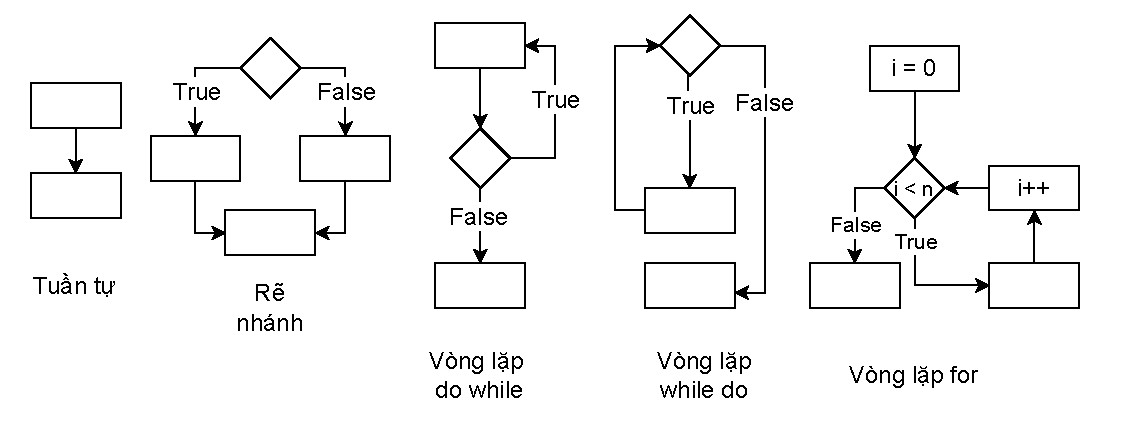
\includegraphics[width=\textwidth]{figures/cfg-control.pdf}
%  		\vspace*{-7mm}
% 		\caption{Các cấu trúc điều khiển phổ biến trong TypeScript}
% 		\label{cau-truc-dieu-khien}
% \end{figure}

% Hình~\ref{cau-truc-dieu-khien} mô tả các cấu trúc điều khiển chính có trong TypeScript được mô phỏng dưới dạng các đỉnh của CFG, bao gồm có cấu trúc điều khiển tuần tự, rẽ nhánh, vòng lặp \textit{for}, vòng lặp \textit{do…while}, vòng lặp \textit{ while…do}.

% \section{Các độ đo kiểm thử}
% Các độ đo kiểm thử thường được xác định là các quy tắc hoặc yêu cầu mà một tập hợp dữ liệu kiểm thử cần đáp ứng \cite{coverage_criteria}. Có một số độ đo phổ biến là bao phủ hàm (function coverage), bao phủ câu lệnh (statement coverage) và bao phủ nhánh (branch coverage). Bao phủ hàm là độ đo dễ đạt được nhất trong ba tiêu chí bao phủ này. Nó được đo bằng tỷ lệ phần trăm các hàm hoặc phương thức đã thực thi trên tổng số các hàm/phương thức có trong mã nguồn thử nghiệm. Bởi vì một hàm được thực thi có thể chứa các đoạn chưa được thực thi như các câu lệnh và các nhánh, một số lỗi bên trong một hàm có thể không được xem xét. Để giải quyết vấn đề này, quá trình kiểm tra phải được thực hiện với cả phạm vi bao phủ của câu lệnh và phạm vi bao phủ nhánh. Liên quan đến bao phủ câu lệnh, nó được biểu thị bằng tỷ lệ phần trăm các câu lệnh được thực thi trong tổng số các câu lệnh thuộc phạm vi kiểm thử. Nếu độ phủ câu lệnh đạt 100\%, thì bao phủ hàm/phương thức cũng đạt đến 100\%. Tuy nhiên, nó không thể xác nhận rằng tất cả các nhánh của điều kiện đều được thực thi. Vì vậy, độ phủ nhánh được đề xuất để đánh giá quá trình thử nghiệm một cách toàn diện hơn. Nó được đo bằng phần trăm các nhánh được thực thi trên tất cả các nhánh thuộc phạm vi kiểm thử. Nếu việc thực thi kiểm thử đạt được bao phủ nhánh tối đa, có thể đảm bảo rằng bao phủ câu lệnh và hàm cũng đạt đến giá trị lớn nhất. Vì vậy, bao phủ nhánh được sử dụng là độ đo cơ bản để đánh giá bộ dữ liệu kiểm thử.

% Công thức tổng quát để tính độ phủ theo các độ đo của $n$ tệp được trình bày trong Công thức \ref{coverage_equation}:
% \begin{equation} \label{coverage_equation}
% \begin{split}
%         e_c &= f(c, tested\ files) \\
%         &= \frac{\sum_{i=1}^n e_{i_c}}
%         {\sum_{i=1}^n t_{i_c}}*100 \\
%  \end{split}
% \end{equation}
% ,trong đó: $c$: loại độ đo bao phủ, bao gồm bao phủ hàm (\textit{function coverage}), bao phủ câu lệnh (\textit{statement coverage}), bao phủ nhánh (\textit{branch coverage})\\
% $e_{i_c}$: số lượng các thành phần được thực thi theo từng độ đo $c$ trong tệp thứ $i$. Thành phần được coi là các hàm, câu lệnh, và nhánh trong mã nguồn kiểm thử. \\
% $t_{i_c}$: số lượng tất cả các thành phần theo độ đo $c$ trong tệp thứ $i$

% Các tiêu chí bao phủ này được sử dụng để đánh giá hiệu quả của phương pháp được đề xuất trong việc tạo dữ liệu thử nghiệm. Nếu độ phủ tăng lên, nhiều thành phần trong mã nguồn được thực thi. Trong trường hợp các độ phủ không đạt 100 \%, các vấn đề sau có thể gặp phải. Thứ nhất, dữ liệu kiểm thử không thực thi toàn bộ các thành phần có trong mã nguồn. Do đó, có thể có một số lỗi tiềm ẩn không được phát hiện. Mặt khác, mã nguồn có thể chứa những câu lệnh không bao giờ có thể thực thi. Các nhà phát triển phải loại bỏ những đoạn mã này để tối ưu kích thước chương trình, tránh thực hiện các hành vi không đúng hoặc đơn giản hóa cấu trúc chương trình.

% % Trong kiểm thử hộp trắng nói chung và kiểm thử dòng điều khiển nói riêng, bài toán kiểm thử là sinh được bộ dữ liệu kiểm thử sao cho thỏa mãn các tiêu chuẩn cho trước. Các tiêu chuẩn này đã được thống nhất và định nghĩa bằng văn bản trong ISO \cite{iso_coverage}. Công thức tính toán độ đo theo các tiêu chuẩn này dựa trên mức độ bao phủ của chương trình với một tập dữ liệu kiểm thử cho trước. Tập dữ liệu kiểm thử có độ phủ cao sẽ đáng tin cậy hơn tập dữ liệu kiểm thử có độ phủ thấp. Mục tiêu là tập dữ liệu kiểm thử có số lượng tối thiểu nhưng đạt được độ phủ tối đa. Hiện nay, có nhiều tiêu chuẩn bao phủ khác nhau được sử dụng. Độ phủ của mỗi tiêu chuẩn đánh giá đều có công thức tính riêng nhưng về cơ bản sẽ được tính bằng tỉ lệ thành phần được kiểm thử trên tổng số các thành phần cần kiểm thử. Thành phần ở đây có thể là câu lệnh, nhánh chương trình, điểm quyết định, điều kiện con hoặc sự kết hợp giữa chúng. Độ đo này giúp các kỹ thuật viên kiểm soát và quản lý quá trình kiểm thử tốt hơn, có thể kiểm tra lại thành phần không được chạy qua hoặc bổ sung thêm dữ liệu kiểm thử trong trường hợp độ phủ thấp. Dưới đây là ba độ đo kiểm thử được sử dụng nhiều trong quy trình kiểm thử phần mềm \cite{Lee03}.
% % \begin{itemize}
% %     \item Độ phủ câu lệnh (statement coverage): mỗi câu lệnh được đi qua ít nhất một lần sau khi chạy bộ dữ liệu kiểm thử.
% %     \item Độ phủ nhánh (branch coverage): nhánh đúng và nhánh sai của mỗi đỉnh điều kiện có trong đồ thị dòng điều khiển được đi qua ít nhất một lần sau khi chạy bộ dữ liệu kiểm thử.
% %     \item Độ phủ điều kiện con (Modified Condition/Decision Coverage - MC/DC): các điều kiện con thuộc các đỉnh điều kiện phức tạp đều được thực hiện cả hai nhánh đúng và nhánh sai ít nhất một lần mỗi nhánh sau khi chạy bộ dữ liệu kiểm thử.
% % \end{itemize}

% % \section{Đường kiểm thử}
% % Bộ dữ liệu kiểm thử sinh ra dành cho một hàm bao gồm nhiều dữ liệu kiểm thử. Mỗi dữ liệu kiểm thử là một bộ giá trị đầu vào của tham số. Với một bộ giá trị đầu vào, chương trình của hàm sẽ chạy qua một số câu lệnh và dừng lại khi tới điểm kết thúc. Tập hợp các câu lệnh theo thứ tự thực hiện tạo thành một đường đi. Những đường đi được chọn để sinh dữ liệu kiểm thử  được gọi là đường kiểm thử. Để thống nhất khái niệm sử dụng trong suốt khóa luận, Định nghĩa 2.4 mô tả tổng quát một đường kiểm thử. Mỗi đường kiểm thử có thể bao gồm đầy đủ các câu lệnh khai báo, gán giá trị, khởi tạo và câu lệnh rẽ nhánh. Các đường đi khác nhau sẽ khác nhau ở số lượng, danh sách và thứ tự thực hiện các câu lệnh. Việc sinh dữ liệu kiểm thử tương ứng với đường kiểm thử chính là tìm kiếm bộ giá trị đầu vào sao cho khi thực thi, các nút điều kiện của đường đi đều được thỏa mãn. Trong thực tế, số lượng đường đi của chương trình có thể rất lớn dẫn đến việc sinh bộ dữ liệu kiểm thử cho tất cả các đường đi là không thể. Vì vậy, một số đường đi được chọn để sinh dữ liệu kiểm thử nhằm đáp ứng tiêu chí về độ phủ được gọi là tập đường kiểm thử.\\
% % \textbf{Định nghĩa 2.1}: Đường kiểm thử là một đường đi từ điểm bắt đầu đến điểm kết thúc của CFG, được biểu diễn bằng tập hợp các đỉnh từ $v_1$  đến $v_n$ sao cho cứ hai đỉnh cạnh nhau thì có cạnh nối theo hướng từ trái qua phải. Nếu cạnh ($v_i$, $v_j$) là nhánh sai thì biểu thức điều kiện tại đỉnh $v_i$ được viết dưới dạng phủ định $!v_i$.

% % Để có thể sinh được bộ dữ liệu kiểm thử thỏa mãn yêu cầu về tiêu chuẩn bao phủ, việc lựa chọn tập kiểm thử là một công đoạn không thể thiếu. Tuy nhiên, có hai vấn đề chúng ta cần phải đối mặt:
% % \vspace{-0.5cm}
% % \begin{itemize}
% %     \item Tính khả thi của đường đi: Một đường kiểm thử gọi là có khả khi nếu tồn tại một dữ liệu kiểm thử sao cho khi thực thi trong môi trường thật, tất cả các đỉnh của đường đi được duyệt qua. Ngược lại, đường kiểm thử gọi là không khả thi.
% %     \item 	Sự bùng nổ đường đi: với một hàm có kích thước lớn, nhiều vòng lặp hoặc các lệnh rẽ nhánh phức tạp, số lượng đường đi của chương trình có thể rất lớn. Việc sinh dữ liệu kiểm thử cho tất cả các đường đi để chắc chắn đạt độ phủ 100\% là không thể.
% % \end{itemize}
% % Mục tiêu của khóa luận này là xây dựng công cụ đầu tiên hỗ trợ sinh dữ liệu kiểm thử cho TypeScript, bắt đầu thử nghiệm với các hàm TypeScript kích thước vừa phải. Vì vậy, tập đường kiểm thử được lựa chọn là tập các đường đi có thể có của chương trình. Trong trường hợp tất cả các đường đi đều khả thi, độ bao phủ nhánh có thể đạt được là 100\%.

% % \section{Thư viện sử dụng}

% % \subsection{Thư viện phân tích mã nguồn TypeScript ``ts-morph''}
% % Phương pháp sinh dữ liệu kiểm thử tự động được đề xuất trong khóa luận này dựa trên việc thao tác với CFG của hàm. Việc xây dựng CFG như thế nào sẽ tùy biến theo từng tình huống bài toán. Đặc biệt đối với một ngôn ngữ mới như TypeScript, hiện tại không có thư viện nào có thể hỗ trợ giải quyết tác vụ này. Vì vậy, quá trình này được thực hiện thủ công dựa trên kỹ thuật phân tích mã nguồn và thiết kế cấu trúc dữ liệu mô hình hóa sao cho phù hợp với bài toán kiểm thử hiện tại. Phân tích mã nguồn thành cây cú pháp trừu tượng (Abstract Syntax Tree - AST) giúp việc xây dựng CFG trở nên đơn giản hơn. AST là một cây đại diện cho cấu trúc cú pháp trừu tượng của mã nguồn. Ngôn ngữ lập trình khác nhau có AST khác nhau.  Mỗi nút của cây biểu thị một cấu trúc có trong mã nguồn. AST thường được xây dựng bởi chính trình phân tích cú pháp của ngôn ngữ tương ứng trong quá trình biên dịch. Đối với các ngôn ngữ lâu đời, việc này có thể được thực hiện bởi một số thư viện khác. Do TypeScript là một ngôn ngữ mới nên chưa có công cụ nào hỗ trợ phân tích mã nguồn thành AST. Vì vậy, khóa luận này sử dụng chính trình biên dịch ngôn ngữ TypeScript của Microsoft để phân tích nội dung hàm. ``ts-morph''\footnote{\url{https://github.com/dsherret/ts-morph}} là một thư viện mở rộng từ trình biên dịch TypeScript, cung cấp các giao diện lập trình ứng dụng (Application Programming Interface - API) hỗ trợ người dùng có một cách dễ dàng hơn để điều hướng chương trình và thao tác với mã TypeScript.
% % Với sự hỗ trợ của ``ts-morph'', người sử dụng có đầy đủ các API để trích xuất thông tin cần thiết từ mã nguồn.  Các khối lệnh của thân hàm và các biểu thức  điều kiện đều có thể dễ dàng có được thông qua việc duyệt các đỉnh, hay gọi là $node$ của AST. Ngoài ra, thư viện cung cấp giao diện\footnote{\url{https://TypeScript-ast-viewer.com/}} để người dùng có thể theo dõi kết quả dưới dạng hình cây rất trực quan và dễ nhìn. Từ đó, việc thao tác với AST trở nên dễ dàng hơn.

% % %  Đối với TypeScript, các cấu trúc này có thể là lớp, hàm, thuộc tính, tham số, câu lệnh, v.v.

% % \subsection{Bộ giải hệ ràng buộc Z3}
% % Công cụ sinh dữ liệu kiểm thử cho mỗi đường kiểm thử bằng cách giải hệ ràng buộc ứng với tập các đỉnh điều kiện. Giải hệ ràng buộc nghĩa là quá trình tìm ra giải pháp cho một tập hợp các ràng buộc áp đặt bởi các phép toán điều kiện mà các biến phải thỏa mãn \cite{ref-constraints}. Do đó, một giải pháp là một tập hợp các giá trị cho các biến thỏa mãn tất cả các ràng buộc, đó là một điểm trong vùng khả thi.
% % Hiện nay, có nhiều thư viện, công cụ hỗ trợ việc giải hệ trong đó nổi bật là bộ giải Z3. Bộ giải Z3 được xây dựng chủ yếu bằng ngôn ngữ C++. Các ràng buộc cần được chuyển sang dạng chuẩn của Z3 để công cụ có thể tính toán và giải nghiệm. Z3 có thể giải hệ ràng buộc của các số nguyên, số thực, mảng và hàm tượng trưng. Đặc biệt trong phiên bản 4.8, bộ giải Z3 hỗ trợ giải một số ràng buộc liên quan đến chuỗi (string) \cite{z3_str_paper}. Điều này giúp việc tìm kiếm dữ liệu kiểm thử có tham số đầu vào kiểu chuỗi trở nên đơn giản hơn. Để có thể sử dụng Z3 giải nghiệm, bộ ràng buộc được lưu trong tệp và khởi chạy tiến trình bằng dòng lệnh:
% % \vspace{0.5cm}
% % \begin{lstlisting}
% % z3 -smt2 <file name>.smt2
% % \end{lstlisting}
% % Mã nguồn~\ref{constraints-file-example} là ví dụ một tệp constraints.smt2 hợp lệ làm đầu vào cho bộ giải Z3. Trong tệp, các biến sử dụng cần được khai báo bằng cú pháp \textit{declare-fun}. Sau đó, lệnh \textit{assert} được sử dụng để thêm các ràng buộc của hệ. Để kiểm tra hệ ràng buộc có nghiệm hay không, lệnh \textit{check-sat} được gọi. Kết quả trả về là \textit{sat} nếu có nghiệm và \textit{unsat} trong trường hợp không có nghiệm. Tập các giá trị của các biến thỏa mãn hệ ràng buộc được hiển thị bằng lệnh \textit{get-model}. Trong ví dụ này, hệ ràng buộc sử dụng ba biến tham số đầu vào là tvw\_s,  tvw\_a, tvw\_b và có ba ràng buộc được thêm vào câu lệnh \textit{assert} trong tệp \textit{constraints.smt2}. Mã nguồn~\ref{z3-result-example} là kết quả tương ứng sau khi giải hệ. Trong đó, các giá trị của các biến tìm được là  tvw\_a = 12,  tvw\_b = 11,  tvw\_s = "\textbackslash x00\textbackslash x00\textbackslash x00\textbackslash x00\textbackslash x00". Như vậy, bộ giá trị (a, b, s) = \{12, 11, "\textbackslash x00\textbackslash x00\textbackslash x00\textbackslash x00\textbackslash x00"\} là một nghiệm của hệ ràng buộc.
% % Nếu áp dụng với một đường kiểm thử cụ thể, các biến được khai báo trong hệ ràng buộc là các biến gọi đến trong các câu lệnh. Các đỉnh điều kiện sẽ được biểu diễn qua những biến này và chuẩn hóa thành những ràng buộc của hệ. Kết quả giải hệ là một dữ liệu kiểm thử thỏa mãn đường đi tương ứng. Trong trường hợp hệ ràng buộc của tất cả các đường đi đều giải được bỏi bộ giải Z3, tập các dữ liệu kiểm thử thu được phủ 100\% đường đi của CFG.

% % \vspace{0.5cm}
% % \begin{lstlisting}[caption=Ví dụ nội dung tệp đầu vào cho bộ giải Z3, label=constraints-file-example,captionpos=b]
% % (set-option :timeout 5000)
% % (declare-fun tvw_s () String)
% % (declare-fun tvw_a () Int)
% % (declare-fun tvw_b () Int)
% % (assert (> a b))
% % (assert (> b 10))
% % (assert (not (> (+ (str.len tvw_s) 1) 10)))
% % (check-sat)
% % (get-model)
% % \end{lstlisting}

% % \begin{lstlisting}[caption=Ví dụ kết quả giải hệ của Z3, label=z3-result-example, captionpos=b]
% % sat
% % (model
% %   (define-fun tvw_s () String
% %     "\x00\x00\x00\x00\x00")
% %   (define-fun tvw_b () Int
% %     11)
% %   (define-fun tvw_a () Int
% %     12)
% % )

% % \end{lstlisting}

% % \subsection{Mocha và Istanbul}
% % Để kiểm tra độ phủ đạt được với bộ dữ liệu kiểm thử đã được sinh tự động, công cụ có sử dụng Mocha trong việc thực thi mã nguồn. Mocha (Mocha Test Framework) là một bộ công cụ hỗ trợ kiểm thử dành cho JavaScript giàu tính năng chạy trên Nodejs và trong trình duyệt, giúp cho việc kiểm tra bất đồng bộ trở nên đơn giản và thú vị \cite{ref-mocha}. Các quy trình thực thi kiểm thử thực hiện bởi Mocha chạy ổn định, cho phép báo cáo linh hoạt và chính xác. Mocha có thể áp dụng với TypeScript thông qua một số bước cài đặt kỹ thuật. Ngoài ra,  Mocha cũng có thể kết hợp với một số thư viện để xuất báo cáo kiểm tra độ phủ (test coverage report). Ngoài việc cung cấp chức năng chạy kiểm thử với thao tác bằng tay, Mocha còn kèm theo bộ API để vận hành các bài kiểm tra tự động. Mocha có rất nhiều tính năng tuyệt vời, trong đó có một số tính năng nổi bật được kể đến là:
% % \begin{itemize}
% %     \item Hỗ trợ bất đồng bộ đơn giản
% %     \item Cung cấp đa dạng báo cáo
% %     \item Có thể chạy trong trình duyệt
% %     \item Tương thích với nhiều thư viện xác nhận (assertion library) Javascript
% %     \item Tương thích với mô hình phát triển phần mềm định hướng hành vi (Behaviour Driven Development - BDD) và mô hình phát triển phần mềm định hướng kiểm thử (Test Driven Development - TDD)
% % \end{itemize}
% % Với sự hỗ trợ của Mocha, các tệp kiểm thử được thực thi một cách nhanh chóng. Kết quả chạy kiểm thử được thống kê trực quan với số lượng dữ liệu kiểm thử thành công hay thất bại kèm theo vị trí cụ thể. Từ đó kỹ thuật viên nhanh chóng xác định được dữ liệu kiểm thử bị sai và dễ dàng sửa chữa.

% % Mocha chỉ hỗ trợ quá trình thực thi tệp kiểm thử và thống kê kết quả số lượng dữ liệu kiểm thử thành công hay thất bại. Tuy nhiên, để có thể biết được thống kê độ phủ mà bộ dữ liệu kiểm thử đạt được, Mocha cần kết hợp thêm một số thư viện bên ngoài. trong đó, được sử dụng nhiều nhất phải kể đến thư viện Istanbul \cite{ref-instanbul}. Đây là thư viện hỗ trợ sinh báo cáo độ phủ của quá trình kiểm thử đơn vị với nhiều định dạng khác nhau như HTML, XML, terminal output, JSON, v.v. Người dùng có thể lựa chọn kiểu báo cáo phù hợp với nhu cầu. Công cụ được phát triển trong khóa luận sử dụng báo cáo thể hiện dưới dạng HTML, bao gồm các thông tin về các độ phủ như số lượng hàm, câu lệnh, nhánh được thực thi. Đồng thời, báo cáo cũng nổi bật các đoạn mã không được chạy qua. Từ đó, kỹ thuật viên có thể phát hiện ra  được các đoạn mã không bao giờ được chạy để làm sạch mã nguồn hoặc bổ sung thêm dữ liệu kiểm thử mới để bộ dữ liệu kiểm thử hoàn thiện hơn.